% Tento soubor nahraďte vlastním souborem s obsahem práce.
%=========================================================================
% Autoři: Michal Bidlo, Bohuslav Křena, Jaroslav Dytrych, Petr Veigend a Adam Herout 2019

% Pro kompilaci po částech (viz projekt.tex), nutno odkomentovat a upravit
%\documentclass[../projekt.tex]{subfiles}
%\begin{document}

\chapter{Úvod}

Vstavané systémy sú neoddeliteľnou súčasťou pokroku a všadeprítomných technológií. Integrované systémy sú obvykle vyvíjané a optimalizované pre predom definovaný účel použitia a platformu. Ich vývoj je často náročný. Vyžaduje pochopenie hardvéru na nízkej úrovni, prácu s~referenčnými manuálmi alebo porozumenie dôležitých aspektov operačného systému. Využívanie neurónových sietí prináša vývojárom radu výhod. Od využitia pri vývoji kódu, cez automatizáciu úloh (generovanie dokumentácie, testovanie), až po zabezpečenie určitých bezpečnostných štandardov a kapacitných nárokov (optimalizácia). Výber oblasti integrovaných systémov pre generovanie kódu je motivovaný ich rozsiahlou aplikáciou v~rôznych oblastiach, ako sú automobilový priemysel, zdravotníctvo, priemyselná automatizácia alebo IoT zariadenia. To poskytuje široké spektrum možností pre aplikáciu nástrojov, ktoré budú schopné pomáhať s~vývojom kódu pre integrované systémy.

Súčasný pokrok v~trénovaní veľkých jazykových modelov a v~oblasti generovania kódu umožnil vznik nových nástrojov a techník pre automatizáciu programovania. V~oblasti generovania kódu sa využívajú jazykové modely, ktoré sú trénované na veľkých dátových sadách a sú schopné generovať kód vysokej kvality. Nástroje ako GitHub Copilot alebo Tabnine, ktoré využívajú jazykové modely na generovanie kódu, sú schopné doplňovať kód, navrhovať funkcie, názvy premenných alebo písať popisy funkcií. Tieto nástroje sa tešia veľkej obľube medzi vývojármi, o~čom svedčia aj správy o~ich využívaní v~praxi. GitHub Copilot totiž v~súčasnosti stojí za 46\% nového kódu na platforme GitHub~\cite{githubcopilot}.

Vývoj takto komplexných nástrojov je náročný proces, ktorý si vyžaduje odborné znalosti v~oblasti strojového učenia, veľké množstvo dát a výpočtovú silu. Počet hodín, ktoré je potrebné investovať do trénovania modelu, sa pohybuje v~státisícoch až miliónoch~\cite{li2023starcoder,workshop2023bloom}. Ďalšie zdroje sú vynaložené na vytváranie a správu rozsiahlych dátových sád, na ktorých sa tieto modely učia. Vývoj modelov strojového učenia je preto náročný proces, ktorý si vyžaduje nielen odborné znalosti a skúsenosti v~oblasti strojového učenia, ale aj značné zdroje.

Rozvoj v~tejto oblasti je aj napriek týmto náročnostiam z~veľkej časti otvorený a orientovaný na komunitu. Vývojári z~celého sveta prispievajú k~vývoju nových modelov, techník a nástrojov, ktoré sú zdieľané s~komunitou. Tento prístup umožňuje rýchlejší vývoj nových technológií a nástrojov, ktoré sú následne dostupné pre širokú verejnosť. Vývojári preto nemusia vytvárať vlastné modely, ale môžu využiť existujúce modely a techniky, ktoré sú dostupné ako open-source projekty. Tento prístup umožňuje adaptovať predtrénované modely (pretrained language model, PLM) pre špecifické účely a využiť ich v~praxi.

V~tejto práci popisujem modely \MC{} a \MCfim{} a dátovú sadu, ktorú som pripravil. Modely \MC{} a \MCfim{} sú zamerané na generovanie kódu pre integrované systémy a sú trénované na dátach špecifických pre túto oblasť. V~práci popisujem zbieranie dát pre nový korpus zdrojových kódov, proces a techniky trénovania modelov. Analyzoval som výsledky modelov s~cieľom poskytnúť prehľad o~ich schopnostiach.

\noindent V~práci sa zameriavam na nasledujúce ciele:
\begin{itemize}
    \item Zbieranie dát z~verejne dostupných repozitárov na platforme GitHub.
    \item Príprava dátových sád pre trénovanie jazykových modelov.
    \item Trénovanie jazykových modelov na dátach z~oblasti integrovaných systémov.
    \item Vyhodnotenie výsledkov trénovania modelov.
\end{itemize}

V~kapitole~\ref{chap:neuron} popisujem základné princípy neurónových sietí a ich využitie v~oblasti strojového učenia. Začínam základným modelom neurónu a pokračujem hlbokými neurónovými sieťami. Tieto koncepty sú kľúčové pre pochopenie architektúry transformer, ktorá je hlavným objektom záujmu tejto práce. Popisujem ju v~kapitole~\ref{chap:transformer}. V~kapitole~\ref{chap:nlp} sa zameriavam na úlohu spracovania prirodzeného jazyka, generovanie kódu a rozdiely medzi prirodzeným a programovacím jazykom. V~kapitole~\ref{chap:training} popisujem základné princípy trénovania jazykových modelov a techniky, ktoré sa používajú pri trénovaní a evaluácií modelov. V~kapitole~\ref{chap:survey} poskytujem prehľad súčasných riešení v~danej oblasti a diskutujem o~ich výhodách a nevýhodách. V~kapitole~\ref{chap:implementation} popisujem proces zbierania dát, prípravu dátovej sady, trénovanie modelov \MC{} a \MCfim{} a evaluáciu výsledkov. Kapitola~\ref{chap:conclusion} uzaviera prácu sumarizáciou dosiahnutých výsledkov. Zamýšľa sa nad možnosťami rozšírenia dátovej sady a navrhuje smer, ktorým by sa mohlo uberať ďalšie výskumné úsilie.

\chapter{Základy neurónových sietí}\label{chap:neuron}

Prvá kapitola sa zameriava na základné princípy neurónových sietí a ich využitie v~oblasti strojového učenia. Začína popisom základného modelu neurónu, ktorý je základnou stavebnou jednotkou neurónových sietí. Nasledujú hlboké neurónové siete, ktoré predstavujú rozšírenie základného modelu a umožňujú modelom učiť sa zložité vzory v~dátach. Tieto koncepty sú kľúčové pre pochopenie architektúry transformera, ktorý je objektom záujmu tejto práce.

\section{Model neurónu}

Základnou funkčnou jednotkou ľudskej nervovej sústavy je bunka nazývaná neurón. Neurón, ktorý je na obrázku~\ref{fig:neuron}, sa skladá z~teľa bunky (soma), vodivých výbežkov (niekoľko vstupných -- dendridy a jeden výstupný -- axón, ktoré slúžia na prijímanie, resp. vysielanie elektrických vzruchov) a synapsií (majú pamäťovú funkciu a vyjadrujú priechodnosť pre vstupné vzruchy). 

\begin{figure}[!ht]
    \centering
    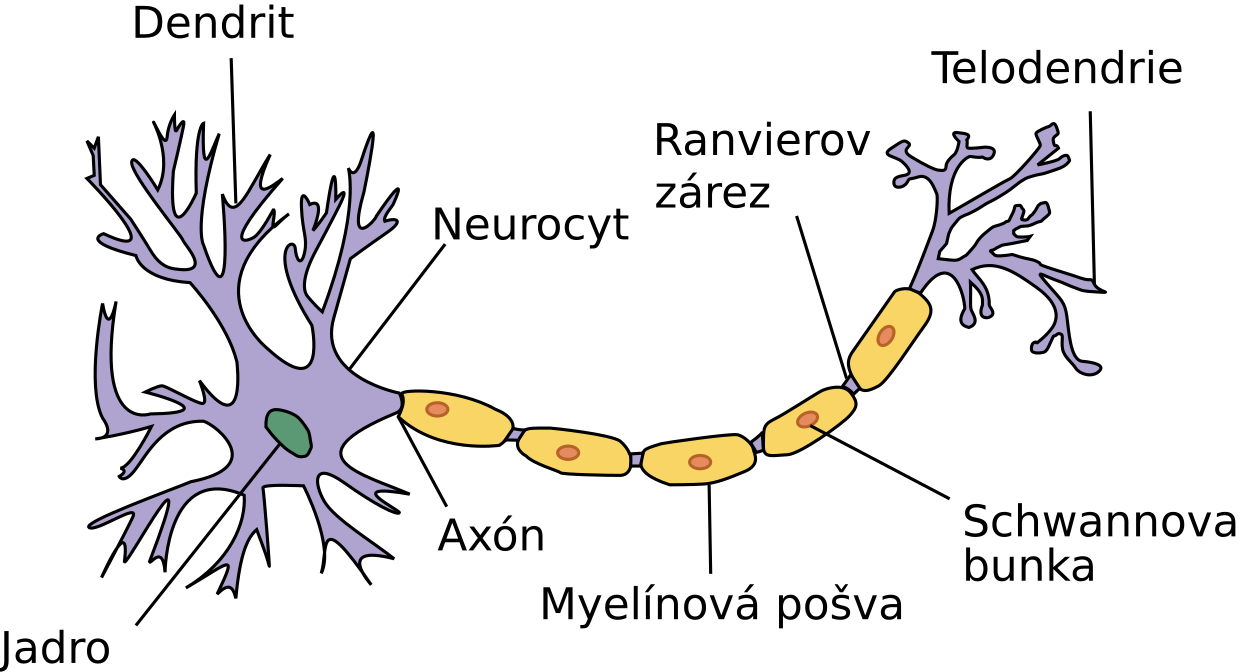
\includegraphics[width=0.7\textwidth]{obrazky/Neuron_slk.png}
    \caption{Schéma biologického neurónu. Prebrané z~\cite{wiki:neuron}.}
    \label{fig:neuron}
\end{figure}

Prvý formálny model neurónu predstavili v~r.\,1943 W.\,S.\,McCulloch a W.\,Pitts~\cite{McCulloch1990}. Tento prvotný McCullochov-Pittsov neurón nebol schopný učiť sa a fungoval ako binárna prahová funkcia, ktorá berie vstupy, aplikuje váhy a vytvára binárny výstup založený na prahovej hodnote. Dôležitý prelom dosiahol F.\,Rosenblatt v~roku 1962 s~jeho modelom neurónu, ktorý nazval \textsc{Perceptrón}. Rosenblatt navrhol algoritmus učenia, ktorý umožnil perceptrónu prispôsobovať svoje váhy na základe chýb v~predikciách. Týmto spôsobom vznikli prvé jednovrstvové učiace sa neurónové siete.

\begin{figure}[!ht]
    \centering
    \begin{tikzpicture}[
        % Styles
        node/.style={circle, draw, thick, minimum size=1cm},
        sum/.style={circle, draw, thick, minimum size=1.5cm},
        arrow/.style={-Stealth, thick},
    ]
    
        % Uzly
        \node[node] (bias) at (3,0) {$\theta$};
        \node[node] (x1) at (0,0) {$x_1$};
        \node[node] (x2) at (0, -1.2) {$x_2$};
        \node[node] (x3) at (0,-2.4) {$x_3$};
        \node (dots) at (0,-3.2) {$\vdots$};
        \node[node] (xn) at (0,-4.2) {$x_n$};
        \node[sum] (sum) at (3,-2.4) {$\sum$};
        \node[node] (function) at (6,-2.4) {$f$};
        \node[node] (output) at (9,-2.4) {$y$};

        % Spoje
        \draw[arrow] (x1) -- node[above] {$w_1$} (sum);
        \draw[arrow] (x2) -- node[above] {$w_2$} (sum);
        \draw[arrow] (x3) -- node[above] {$w_3$} (sum);
        \draw[arrow] (xn) -- node[above] {$w_n$} (sum);
        \draw[arrow] (bias) -- (sum);
        \draw[arrow] (sum) -- (function);
        \draw[arrow] (function) -- (output);
        
        % Popis
        \node[below=0.5cm] at (xn) {Vstupy};
        \node[below=0.8cm] at (sum) {Sumácia};
        \node[below=0.5cm] at (function) {\parbox{3cm}{\centering Aktivačná\\funkcia}};
        \node[right=0.5cm] at (bias) {Bias};
        \node[below=0.5cm] at (output) {Výstup};
        
    \end{tikzpicture}
    \caption{Perceptrón -- základný model umelého neurónu s~$n$ vstupmi a váhami, jedným výstupom a prahom citlivosti.}
    \label{fig:perceptron}
\end{figure}

Operácie vykonávané perceptrónom, podľa knihy~\cite{Novak1998}, možno rozdeliť na synaptické operácie (konfluencia) a somatické operácie (agregácia, prahovanie a nelineárne zobrazenie), ktoré spoločne poskytujú základný pohľad na fungovanie perceptrónu.

\subsection*{Synaptické operácie}

Do perceptrónu vstupuje n-rozmerný vektor vstupných signálov $x \in R^n$. Operácia konfluencie (splinutia) kombinuje vstupné signály s~uloženými synaptickými váhami, ktoré sú reprezentované váhovým vektorom $w \in R^n$. Tieto váhy odrážajú dôležitosť jednotlivých vstupov pre výsledný výstup neurónu.

\subsection*{Somatické operácie}

Následne sa výsledok konfluencie agreguje na skalárnu hodnotu. V~základnom modeli je možné túto agregáciu nahradíť sumáciou zložiek výsledku konfluencie. Ďalej nasleduje prahovanie a nelineárne zobrazenie. Ak je výsledok sumácie menší ako hodnota prahu (bias) $\theta$, na výstupe sa zobrazí hodnota neaktívneho stavu. V~opačnom prípade, ak výsledok prekročí hodnotu prahu, aktivuje sa neurón a výstup sa získa prostredníctvom nelineárnej aktivačnej funkcie $f$. Tento mechanizmus umožňuje perceptrónu realizovať nelineárne transformácie vstupných signálov, čím zvyšuje jeho schopnosť modelovať komplexné vzťahy. Výstup perceptrónu možno matematicky vyjadriť ako:
\begin{equation}
    y = f(\theta + \sum_{i=1}^{n}x_i \cdot w_i)
\end{equation}


\subsection{Aktivačná funkcia}

Aktivačná funkcia je nelineárna funkcia, ktorá sa aplikuje na výsledok sumácie vstupov a váh. Oproti binárnej prahovej funkcií, ktorá bola pôvodne používaná, obor hodnôt aktivačnej funkcie je spojitý a umožňuje modelu aproximovať zložitejšie vzory v~dátach. Spojitý obor hodnôt umožňuje modelu odpovedať na malé zmeny vstupov malými zmenami výstupov, čo je dôležité pre učenie modelu. Výber vhodnej aktivačnej funkcie závisí od konkrétnej úlohy, ktorú model rieši. Medzi najpoužívanejšie aktivačné funkcie patria:
\begin{itemize}
    \item \textbf{Sigmoidálna funkcia} -- Sigmoidálna aktivačná funkcia je vyhladená verzia binárnej prahovej funkcie, ktorá transformuje vstup na hodnotu medzi 0 a 1. Táto funkcia sa často používa na binárne klasifikačné úlohy, kde model predikuje pravdepodobnosť príslušnosti k~jednej z~dvoch tried. Sigmoidálna funkcia zohrala dôležitú úlohu pri vývojí algoritmu spätného šírenia, ktorý je základným algoritmom pre trénovanie hlbokých neurónových sietí, ale v~súčasnosti sa používa menej kvôli problémom s~gradientom pri trénovaní hlbokých sietí.

    $$f(x) = \frac{1}{1 + e^{-x}}$$
    
    \item \textbf{Hyperbolický tangens (tanh)} -- Hyperbolický tangens je podobný sigmoidálnej funkcii, ale obor hodnôt funkcie je medzi -1 a 1. Táto funkcia sa často používa na regresné úlohy, kde model predikuje hodnotu v~určitom rozsahu. Hyperbolický tangens má výhodu oproti sigmoidálnej funkcii v~posunutí, stredná hodnota je 0, čo zjednodušuje učenie modelu.

    $$f(x) = \tanh(x) = \frac{e^{2x}-1}{e^{2x}+1}$$
    
    \item \textbf{Rectified Linear Unit (ReLU)} -- Jedná sa o~najčastejšie využívanú aktivačnú funkciu implementovanú v~skrytých vrstvách neurónovej siete. Na rozdiel od \textup{tanh} alebo sigmoidálnej funkcie je rýchlejšia, pretože implementuje jednoduchšie operácie.
    
    $$f(x) = \max(0, x) = \frac{x + \left|x\right|}{2}$$
    
    Ďalšou výhodou je, že spĺňa podmienku $ f(\delta z) = \delta f(z)$ a patrí do skupiny aktivačných funkcií, ktoré nie sú závislé od škálovania vstupu.

    Jednou z~nevýhod \textup{ReLU} je, že sa neuróny môžu dostať do stavu, v~ktorom sa stanú neaktívne pre \uv{všetky} vstupy -- varianta miznúceho gradientu. \textup{ReLU} má niekoľko variant, ktoré ponúkajú riešenia -- \textup{GELU}, \textup{leaky ReLU}, \textup{SiLU}, \textup{Softplus} a iné.
    
    \item \textbf{Softmax} -- Softmax je aktivačná funkcia, ktorá sa používa na klasifikačné úlohy s~viacerými triedami. Funkcia transformuje vstup na pravdepodobnostné rozdelenie, ktoré vyjadruje pravdepodobnosť príslušnosti k~jednej z~$n$ tried.

    $$f(x) = \frac{e^{x_i}}{\sum_{j=1}^{n}e^{x_j}}$$
    
\end{itemize}

\section{Hlboké neurónové siete}

V~tejto sekcií čerpám zo zdrojov~\cite{enwiki:1222136552, enwiki:1222140497}. Schopnosti perceptrónu s~jednou vrstvou sú obmedzené na riešenie lineárne separovateľných problémov. To znamená, že dokáže korektne klasifikovať dáta len v~prípadoch, kde existuje lineárna hranica medzi rôznymi triedami alebo kategóriami. Pre riešenie zložitejších problémov, kde dáta nie sú lineárne separovateľné alebo kde vzťahy medzi vstupmi a výstupmi sú komplexnejšie, je potrebné použiť sofistikovanejšie modely. Teorém univerzálnej aproximácie~\cite{enwiki:1221184532} je teoretický základom toho, ako fungujú hlboké neurónové siete. Tvrdí, že neurónová sieť s~aspoň jednou skrytou vrstvou (angl. hidden layer), ktorá sa skladá z~dostatočného množstva umelých neurónov s~nelineárnymi aktivačnými funkciami, je schopná aproximovať ľubovoľnú spojitú funkciu s~ľubovoľnou presnosťou. Hlboká neurónová sieť (Deep Neural Network, DNN) predstavuje rozšírenie perceptrónu s~viacerými vrstvami, ktoré umožňujú modelu učiť sa komplexné vzorce a vytvárať abstraktné reprezentácie vstupov. Hlboké neurónové siete sú schopné reprezentovať nelineárne vzťahy medzi vstupmi a výstupmi, a tým sa stali kľúčovým nástrojom pre riešenie širokej škály problémov v~oblasti strojového učenia, presnejšie hlbokého učenia (Deep Learning, DL).

V~súčasnej dobe sú hlboké neurónové siete základom pre pokročilé aplikácie v~mnohých oblastiach vrátane spracovania prirodzeného jazyka, počítačového videnia, rozpoznávania reči, a ďalších. Pri implementácii hlbokých neurónových sietí sú kľúčové techniky ako napríklad spätné šírenie chyby (backpropagation), ktoré umožňuje efektívne aktualizovať váhy siete na základe chyby výstupu.

Okrem toho, hlboké učenie využíva rôzne typy architektúr sietí, ako sú konvolučné neurónové siete (Convolutional neural network, CNN) pre vizuálne údaje, rekurentné neurónové siete (Recurrent neural network, RNN) pre sekvenčné dáta, a transformer, ktorý sa čoraz viac používajú v~mnohých oblastiach spracovania prirodzeného jazyka.

% Zdrojový kód obrázku neurónovej siete je adaptovaný zo zdroju https://tikz.net/neural_networks/
\begin{figure}[!ht]
    \centering
    % COLORS
    \colorlet{myred}{red!80!black}
    \colorlet{myblue}{blue!80!black}
    \colorlet{mygreen}{green!60!black}
    \colorlet{myorange}{orange!70!red!60!black}
    \colorlet{mydarkred}{red!30!black}
    \colorlet{mydarkblue}{blue!40!black}
    \colorlet{mydarkgreen}{green!30!black}
    
    % STYLES
    \tikzset{
      >=latex, % for default LaTeX arrow head
      node/.style={thick,circle,draw=myblue,minimum size=22,inner sep=0.5,outer sep=0.6},
      node in/.style={node,green!20!black,draw=mygreen!30!black,fill=mygreen!25},
      node hidden/.style={node,blue!20!black,draw=myblue!30!black,fill=myblue!20},
      node out/.style={node,red!20!black,draw=myred!30!black,fill=myred!20},
      connect/.style={thin,mydarkblue}, %,line cap=round
      node 1/.style={node in}, % node styles, numbered for easy mapping with \nstyle
      node 2/.style={node hidden},
      node 3/.style={node out}
    }
    \def\nstyle{int(\lay<\Nnodlen?min(2,\lay):3)} % map layer number onto 1, 2, or 3
    \begin{tikzpicture}[x=2.2cm,y=1.4cm]
        \readlist\Nnod{3,5,5,5,2} % array of number of nodes per layer
        
        \message{^^J  Layer}
        \foreachitem \N \in \Nnod{ % loop over layers
        \def\lay{\Ncnt} % alias of index of current layer
        \pgfmathsetmacro\prev{int(\Ncnt-1)} % number of previous layer
        \message{\lay,}
        \foreach \i [evaluate={\y=\N/2-\i; \x=\lay; \n=\nstyle;}] in {1,...,\N}{ % loop over nodes
          
          % NODES
          \node[node \n] (N\lay-\i) at (\x,\y) {};
          
          % CONNECTIONS
          \ifnum\lay>1 % connect to previous layer
            \foreach \j in {1,...,\Nnod[\prev]}{ % loop over nodes in previous layer
              \draw[connect,white,line width=1.2] (N\prev-\j) -- (N\lay-\i);
              \draw[connect] (N\prev-\j) -- (N\lay-\i);
              %\draw[connect] (N\prev-\j.0) -- (N\lay-\i.180); % connect to left
            }
          \fi % else: nothing to connect first layer
          
        }
        }
        
        % LABELS
        \node[above=5,align=center,mygreen!60!black] at (N1-1.90) {vstupná\\ vrstva};
        \node[above=2,align=center,myblue!60!black] at (N3-1.90) {skryté vrstvy};
        \node[above=10,align=center,myred!60!black] at (N\Nnodlen-1.90) {výstupná\\vrstva};
        
    \end{tikzpicture}
    \caption[Zjednodušená ilustrácia hlbokej neurónovej siete s~tromi skrytými vrstvami]{Zjednodušená ilustrácia hlbokej neurónovej siete s~tromi skrytými vrstvami.\protect\footnotemark}
    \label{fig:dnn}
\end{figure}

\footnotetext{Vizualizácia neurónovej siete adaptovaná z~\url{https://tikz.net/neural_networks/}.}

\subsection{Spätné šírenie}

Spätné šírenie (angl. backpropagation) predstavuje kľúčový algoritmus používaný na efektívne trénovanie hlbokých neurónových sietí. Jeho základ tvorí metóda gradientného zostupu, ktorá sa systematicky aplikuje na aktualizáciu váh v~sieti s~cieľom minimalizovať chybovosť modelu porovnaním jeho predikcií s~referenčnými výstupnými hodnotami. Spätné šírenie využíva reťazové pravidlo derivácií, ktoré umožňuje efektívne propagovať chyby späť cez sieť a vypočítať gradienty pre každú váhu, čím sa poskytuje presný smer a veľkosť potrebných úprav váh.

Tento proces je výpočtovo intenzívny, pretože vyžaduje výpočet gradientov pre všetky váhy v~sieti, čo v~prípade veľkých modelov predstavuje obrovské množstvo operácií. Preto je spätné šírenie často implementované s~využitím grafických procesorov (GPU), ktoré dokážu výrazne zrýchliť trénovanie vďaka ich schopnosti paralelne spracovávať veľké množstvá dát. Vďaka tejto schopnosti a pokrokom v~oblasti výpočtovej techniky sa spätné šírenie stalo fundamentálnou technikou pre trénovanie hlbokých neurónových sietí, umožňujúc modelom učiť sa komplexné vzorce a funkcie z~rozsiahlych dátových sád.

\chapter{Transformer -- model hlbokého učenia}\label{chap:transformer}

Ako bolo možné vidieť v~predchádzajúcich sekciách, základy neurónových sietí a ich schopnosti učiť sa z~komplexných dátových súborov formujú elementárne kamene moderného strojového učenia. Postupy ako spätné šírenie a aktivačné funkcie, ktoré umožňujú neurónovým sieťam efektívne sa učiť a adaptovať, sú neoceniteľné pre riešenie rozmanitých problémov v~oblasti umelej inteligencie. Hlboké neurónové siete, založené na týchto princípoch, dokázali dosiahnuť významný pokrok v~mnohých aplikáciách, vrátane spracovania prirodzeného jazyka.

V~oblasti neurónových sietí transformery predstavujú revolučnú metódu spracovania prirodzeného jazyka. Na rozdiel od tradičných architektúr, ako sú RNN alebo CNN, transformery využívajú mechanizmy pozornosti (attention) na efektívne zachytenie komplexných vzťahov v~sekvenčných dátach. Možnosť každého slova v~sekvencii vplývať na ostatné slová v~sekvencii umožňuje transformerom excelovať vo vytváraní modelov dlhodobých závislostí, ktoré sú kľúčové pre úlohy ako strojový preklad a generovanie textu. Architektúra kodéru (encoder) a dekodéru (decoder), charakteristická pre transformery, umožňuje spracovanie vstupných sekvencií do abstraktných reprezentácií prostredníctvom kodéru, nasledované generovaním výstupných sekvencií dekodérom. Transformery umožnili vznik rozsiahlych predtrénovaných jazykových modelov, ako je napríklad séria \GPT{} od firmy OpenAI alebo \LLAMA{} od firmy Meta, ktoré preukázali prispôsobivosť pre rôzne oblasti a schopnosť generalizovať naučené vzorce. Schopnosťou prenosu učenia transformery zmenili paradigmu v~porozumení prirodzenému jazyku, otvárajúc cestu k~inovatívnym aplikáciám v~oblasti výskumu a vývoja umelej inteligencie.

V~tejto kapitole sa podrobnejšie pozriem na to, ako transformer využíva tieto koncepty a ako sa architektúra transformera stala kľúčovou technológiou pre generatívne modely v~oblasti spracovania prirodzeného jazyka (NLP). V~tejto kapitole popíšem transformáciu textu, mechanizmus pozornosti, zameriam sa na základné stavebné bloky transformera, ako sú kodér a dekodér, a diskutujem o~ich funkcii a prínosoch.

\section{Tokenizácia}

Tokenizácia je proces transformácie textu na sekvenciu tokenov. Tokeny môžu byť jednotlivé slová, písmená alebo podreťazce, ktoré sú použité na reprezentáciu vstupných dát. Dôležitou črtou tokenizácie je schopnosť rozdeliť text na časti, ktoré majú pre model zmysel. To zahŕňa rozdelenie textu na jeho zložky tak, aby boli zachované sémantické a syntaktické vlastnosti originálneho textu. Existuje niekoľko prístupov k~tokenizácii, ktoré sa odlišujú granularitou a metodikou tokenizácie. Medzi najpoužívanejšie prístupy patria:

\begin{itemize}
    \item \textbf{Tokenizácia na úrovni slov} -- Text je rozdelený na jednotlivé slová, ktoré sú tokenmi. Tento prístup je najpoužívanejší v~prípade, že slová jazyka sú efektívne separovateľné medzerami. 
    \item \textbf{Tokenizácia na úrovni znakov} -- Text je rozdelený na jednotlivé znaky, ktoré sú tokenmi. Tento prístup je vhodný pre jazyky, ktoré nemajú jasne definované separátory slov, alebo napríkald pre úlohy, ktoré analyzujú štruktúru textu na úrovni znakov.
    \item \textbf{Tokenizácia na podreťazce} -- Spojenie predchádzajúcich prístupov, ktoré rozdeľuje text na podreťazce, ktoré sú často používané v~texte. Tento prístup umožňuje modelu pracovať s~neznámymi slovami alebo slovami, ktoré nie sú obsiahnuté v~slovníku.
\end{itemize}

\subsection{BPE tokenizácia}

Byte-Pair Encoding (BPE) je pokročilá metóda tokenizácie na podreťazce, ktorá zohráva kľúčovú úlohu NLP, najmä v~aplikáciách ako strojový preklad a generovanie textu. BPE funguje na princípe postupného spájania znakov alebo reťazcov znakov na základe frekvencie ich výskytu v~dátovej sade, čím sa postupne vytvára optimalizovaný slovník tokenov. Tento proces sa opakuje, kým nie je dosiahnutá požadovaná veľkosť slovníka. Nevýhodou je, že takto naučený model môže mať problém s~neznámymi znakmi, ktoré nie sú obsiahnuté v~slovníku. Tento problém rieši \textsc{byte-level BPE} tokenizácia, ktorá pracuje na úrovni bytov, na nižšej úrovni reprezentácie textu. Počiatočný slovník tak má vždy veľkosť 256 tokenov, ktoré postupne spája do zložitejších tokenov. Tento prístup umožňuje modelu pracovať s~neznámymi znakmi a zároveň zachováva výhody BPE tokenizácie.

\begin{figure}
    \centering
    \includesvg[width=0.8\textwidth]{obrazky/BPE.svg}
    \caption{Proces rozkladu vstupného zdrojového kódu na tokeny. Tokeny môžu byť napríklad kľúčové slová, identifikátory, operátory alebo zátvorky.}
    \label{fig:tokenization}
\end{figure}

Rovnako ako existujú rozdiely medzi prirodzenými a programovacími jazykmi, diskutované v~sekcií~\ref{sec:code_gen}, tokenizácia pre programovacie jazyky vyžaduje špecifické úpravy. Je štandardné, keď je tokenizér trénovaný spolu s~jazykovým modelom na trénovacích dátach z~oblasti, v~ktorej bude model nasadený. Tento prístup umožňuje tokenizáciu, ktorá je špecifická pre konkrétnu doménu, čo môže viesť k~lepším výsledkom. 

\section{Mechanizmus pozornosti}

Mechanizmus pozornosti~\cite{vaswani2023attention} predstavuje fundamentálny koncept v~architektúre transformerov a umožňuje efektívne zachytávať komplexné vzájomné väzby v~sekvenčných dátach. Neurónové siete typu transformer neimplementujú rekurentné prepojenia, ktoré sú charakteristické pre RNN, ale namiesto toho sa spoliehajú výlučne na mechanizmus pozornosti na zachytenie vzájomných vzťahov dát v~sekvencii~\cite{BishopDeepLearning}.


Pozornosť umožňuje pre každú pozíciu v~sekvencii, token, vypočítať váhy pre ostatné pozície. Tieto váhy kvantifikujú mieru, do akej daná pozícia pri generovaní reprezentácie vplýva na ostatné pozície v~sekvencii. Pre ilustráciu toho, na čo slúži pozornosť, uvádzam príklad z~knihy~\cite{BishopDeepLearning}. Slovo \uv{bank}, má v~anglickom jazyku viacero významov. Jedným môže byť breh rieky, druhým je banka, ako finančná inštitúcia, pričom záleží na kontexte, v~ktorom je slovo použité. Na obrázku~\ref{fig:attention_view} je vidieť, ako vplývajú jednotlivé slová na ostatné v~sekvencii. Váhy pozornosti pre slovo "bank" v~kontexte \textit{\uv{I swam accross the river to get to the other bank.}} sú zamerané na slovo \textit{\uv{river}}, zatiaľ čo v~kontexte \textit{\uv{I walked accross the road to get cash from the bank.}} sú zamerané na slovo \textit{\uv{cash}}.

\begin{figure}[!ht]
    \centering
    \includegraphics[width=0.4\textwidth]{obrazky/attention_view1.png}
    \includegraphics[width=0.4\textwidth]{obrazky/attention_view2.png}
    \caption{Vizualizácia naučených váh hláv jednej vrstvy mechanizmu pozornosti modelu \BERT{} s~využitím nástroja~\cite{vig-2019-multiscale}.}
    \label{fig:attention_view}
\end{figure}

\subsection{Samopzornosť}~\label{sec:self-attention}

Na výpočet váh pozornosti sa v~praxi používa mechanizmus nazývaný samopzornosť (self-attention). Samopzornosť umožňuje modelu vypočítať váhy pozornosti pre každú pozíciu v~sekvencii na základe vstupných reprezentácií. V~kontexte samopzornosti sa mechanizmus pozornosti aplikuje na tú istú sekvenciu.

\noindent Fungovanie mechanizmu samopozornosti v~architektúre transformer:
\begin{enumerate}
    \item Každý vstupný vektor $x_i$ je lineárne transformovaný na tri vektory $q_i$, $k_i$ a $v_i$ pomocou naučených váhových matíc $W_Q$, $W_K$ a $W_V$.
    \item Pre každú pozíciu $x_i$ v~sekvencii sú vypočítané váhy pozornosti $a_{ij}$ pre ostatné pozície $x_j$ v~sekvencii na základe vektorov $q_i$ a $k_j$. Skalárny súčin $q_i \cdot k_j$ je následne upravený faktorom $\frac{1}{\sqrt{d_k}}$ a normalizovaný pomocou funkcie softmax, ktorá zabezpečuje, že váhy pozornosti sú nezáporné a ich súčet je rovný jednej.
    \begin{equation}
        a_{ij} = softmax\left(\frac{q_i \cdot k_j}{\sqrt{d_k}}\right)
    \end{equation}
    \item Výsledná reprezentácia $y_i$ pre pozíciu $x_i$ je vypočítaná ako vážená suma vstupných reprezentácií $x_j$ na základe váh pozornosti $a_{ij}$.
    \begin{equation}\label{eq:attention}
        y_i = \sum_{j=1}^{n}a_{ij}v_j
    \end{equation}
\end{enumerate}

Rovnica~\ref{eq:attention} reprezentuje výpočet výslednej reprezentácie $y_i$ pre pozíciu $x_i$ ako váženú sumu vstupných reprezentácií $x_j$, kde váhy pozornosti $a_{ij}$ určujú príspevok každej vstupnej reprezentácie $x_j$ k~výslednej reprezentácii $y_i$. Takto spočítaná pozornosť sa nazýva pozornosť skalárneho súčinu (scaled dot-product attention), pretože váhy pozornosti sú vypočítané ako skalárny súčin vektorov $q_i$ a $k_j$ upravený faktorom $\frac{1}{\sqrt{d_k}}$.

Jedným z~významných prínosov pozornosti je možnosť interpretovať rozhodnutia modelu týkajúce sa dôležitosti rôznych častí vstupných dát. To znamená, že model môže poskytnúť vysvetlenia, prečo určité časti vstupných dát ovplyvňujú jeho rozhodnutia, čo je kritické pre aplikácie, ktoré vyžadujú transparentnosť a interpretovateľnosť. V~praxi sa pozornosť v~transformeroch používa v~rôznych častiach modelu a hrá kľúčovú úlohu vo vytváraní presných a výkonných modelov spracovania prirodzeného jazyka. Mechanizmus samopozornosti sa tak stáva revolučným nástrojom v~oblasti spracovania prirodzeného jazyka a umožňuje dosahovať mimoriadne výsledky v~rôznych úlohách.

\begin{figure}[!ht]
    \centering
    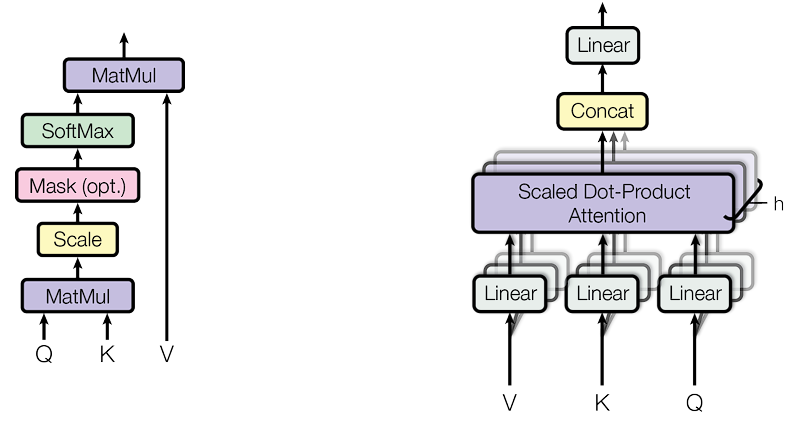
\includegraphics[width=0.8\textwidth]{obrazky/Attention.png}
    \caption{Pozornosť skalárneho súčinu (vľavo) a multi-head pozornosť (vpravo). Prebrané z~\cite{vaswani2023attention}.}
    \label{fig:attention}
\end{figure}

\subsection{Multi-head pozornosť}

Na obrázku~\ref{fig:attention} vidieť, že takto navrhnutých \uv{hláv} pozornosti sa využíva niekoľko paralelne poskladaných. Tento prístup, nazývaný multi-head pozornosť (multi-head attention, MHA), umožňuje modelu zachytiť rôzne aspekty vstupných dát a vytvoriť bohatšie reprezentácie, ktoré sú schopné zachytiť zložité vzťahy v~dátach. Každá hlava pozornosti sa naučí vytvárať rôzne reprezentácie vstupných dát a následne sú tieto reprezentácie spojené do jednej výslednej reprezentácie. Výsledná rovnica pre Multi-head pozornosť je definovaná ako:
\begin{equation}
    MultiHead(Q, K, V~) = Concat(head_1, \cdots, head_h)W^O
\end{equation}

\section{Architektúra transformer}

V~tejto podkapitole je popísaná architektúra transformer, pričom sa čerpá z~práce~\cite{vaswani2023attention}. Architektúra transformer je založená na princípe kodéru a dekodéru. Kodér aj dekodér sa skladajú z~niekoľkých na sebe naskladaných identických vrstiev. Kodér je zodpovedný za reprezentáciu vstupných dát, zatiaľ čo dekodér generuje výstupné dáta na základe reprezentácií vytvorených kodérom a výstupov z~predchádzajúcich vrstiev dekodéra. Architektúra transformer je zobrazená na obrázku~\ref{fig:transformer_architecture}.

\begin{figure}[!ht]
    \centering
    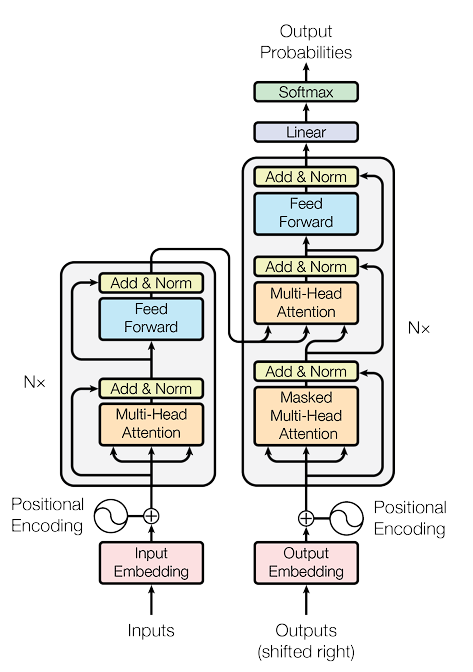
\includegraphics{obrazky/Transformer_architecture.png}
    \caption{Architektúra transformer s~$N$ kodér a dekodér blokmi. Prebrané z~\cite{vaswani2023attention}.}
    \label{fig:transformer_architecture}
\end{figure}

\subsection{Kodér}

Kodér je navrhnutý tak, aby spracoval vstupnú sekvenciu a transformoval ju na sériu vektorových reprezentácií, ktoré obsahujú kontextové informácie z~celého vstupu. Kontextové vektory sú následne použité dekodérom na 
generovanie výstupnej sekvencie.

\noindent Popis fungovania kodéru:
\begin{enumerate}
    \item Vstupná sekvencia tokenov do kodéru je najprv prevedené na spojité vektorové reprezentácie, vrstva vnorenia slov (input embedding), následne sú pripočítané informácie o~poradí jednotlivých tokenov v~sekvencii, pozičné kódovanie (positional encoding). Po inicializácii vstupných vektorových reprezentácií nasleduje spracovávanie sériou $N$ vrstiev kodéru.

    \item Každá vrstva kodéru sa skladá z~dvoch podvrstiev. Prvou je MHA a druhou je plne pozičná plne prepojená dopredná sieť (position-wise fully connected feed-forward network, FFN), ktorá pozostáva z~dvoch lineárnych transformácií, aplikovaných na každú pozíciu sekvencie, a nelineárnej ReLU aktivačnej funkcie.

    \begin{equation}
        FFN(x) = max(0, xW_1 + b_1)W_2+b_2
    \end{equation}
    
    MHA umožňuje kodéru analyzovať vstupné dáta z~rôznych kontextových perspektív, zatiaľ čo dopredná sieť ďalej spracováva výstup mechanizmu pozornosti na generovanie výslednej reprezentácie pre každý token v~sekvencii.

    \item Po každej podvrstve MHA a FFN sú pridané reziduálne spojenia, nasledované normalizačnou vrstvou\footnote{Na rozdiel od pôvodnej architektúry platí, že v~súčasných modeloch sa vykonáva normalizácia pred vrstvami MHA a FFN. Zistilo sa totiž, že pre modeli, ktoré majú 10 a viac vrstiev, sa stáva učenie nestabilné~\cite{takase2023b2t}.}. Tieto komponenty pomáhajú zabrániť problémom s~miznúcim alebo explodujúcim gradientom a zlepšujú stabilitu učenia.
\end{enumerate}

\subsection{Dekodér}

Dekodér sa skladá zo série identických vrstiev, kde každá vrstva prijíma vstupy z~predchádzajúcej vrstvy a poskytuje vstupy pre nasledujúcu vrstvu. Tento proces sa opakuje, až kým nie je dosiahnutý požadovaný výstup alebo dosiahnutá maximálna dĺžka sekvencie.

\noindent Dekodér má podobnú štruktúru ako kodér, ale obsahuje aj zásadné zmeny:
\begin{enumerate}
    \item Podobne ako pre kodér platí, že vstup do dekodéra je najprv transformovaný do vektorového priestoru a skombinovaný s~pozičným kódovaním. Vstupy do kodéru sú obvykle výstupné tokeny, ktoré model generoval v~predchádzajúcich krokoch (autoregresívny prístup).

    \item Prvá MHA vrstva je upravená, aby maskovala budúce informácie, čo znamená, že pri generovaní reprezentácie pre pozíciu $x_i$ v~sekvencii dekodér nemá prístup k~informáciám z~pozícií $x_j$ pre $j > i$. Táto úprava spolu s~posunutím vstupných reprezentácií do dekodéru zabezpečujú, že dekodér generuje reprezentácie iba na základe informácií na pozíciach menších ako $i$.

    \item Stavba dekodéra je rozšírená o~ďalší mechanizmus pozornosti, ktorý umožňuje dekodéru pozerať sa na výstupné reprezentácie vytvorené kodérom. Tento mechanizmus, nazývaný kodér-dekodér pozornosť, umožňuje dekodéru pristúp ku kompletnej reprezentácií vstupných dát z~kodéru a ich využitie pri generovaní výstupných reprezentácií.

    \item Výstupy sú nakoniec prevedené cez lineárnu vrstvu a softmax funkciu, ktorá generuje pravdepodobnosti nasledujúcich tokenov v~sekvencii.
\end{enumerate}


\chapter{Spracovanie prirodzeného jazyka}\label{chap:nlp}

Spracovanie prirodzeného jazyka (Natural Language Processing, NLP) je disciplína umelej inteligencie a lingvistiky, ktorá sa zaoberá spracovaním a analýzou ľudského (prirodzeného) jazyka. Zahŕňa vývoj algoritmov a modelov s~cieľom umožniť výpočtovým systémom porozumieť, interpretovať a generovať ľudský jazyk. Tieto systémy môžu byť aplikované na rôzne úlohy, ako sú rozpoznávanie reči, strojový preklad, analýza sentimentu, generovanie textu a extrakcia informácií.

NLP nie je novým konceptom; jeho korene siahajú už do 40. rokov 20. storočia. V~roku 1950 publikoval Alan Turing vedecký článok, ktorý sa zaoberal otázkou, či stroj môže myslieť~\cite{TURING1950}. Tento článok je považovaný za jeden z~prvých príspevkov k~oblasti umelej inteligencie a NLP. Mimo iného sa v~článku zaoberal aj otázkou, či by mohol stroj porozumieť a generovať ľudský jazyk, respektíve navrhol hru, ktorá sa stala známou ako Turingov test. Tento test sa stal kľúčovým v~oblasti NLP a umelej inteligencie, pretože sa zaoberá otázkou, či je počítač schopný komunikovať s~človekom tak, aby človek nebol schopný rozlíšiť, či komunikuje s~počítačom alebo s~iným človekom. Turingov test je dnes už všeobecne považovaný za nedostatočný pre posúdenie inteligencie, ale výzvy spojené s~nejednoznačnosťou a zložitosť prirodzeného jazyka pretrvávajú.

Slová a frázy často majú viacero významov v~závislosti od kontextu, čo robí ťažké pre počítače presne porozumieť a spracovať jazykové údaje. Okrem toho jazyky prejavujú syntaktické a sémantické varianty, čo viac komplikuje úlohu NLP. S~nástupom strojového učenia a neskôr hlbokého učenia (deep learning) došlo k~dramatickému posunu v~schopnostiach NLP. Modely založené na strojovom učení sa učia zo vzorov v~dátach, čo umožňuje adaptáciu na nové jazykové konštrukcie bez potreby explicitného programovania každej možnej situácie. Hlboké učenie, a najmä neurónové siete, posunuli tieto schopnosti ďalej, umožňujúc modelom učiť sa komplexné vzorce a nuansy jazyka z~obrovských množstiev textových dát. Na riešenie týchto výziev vznikli sofistikované modely ako rekurentné neurónové siete, siete s~dlhou krátkodobou pamäťou (long short-term memory network, LSTMs~\cite{LSTM1997}) a v~posledných rokoch veľmi úspešné modely založené na architektúre transformer. Tieto modely využívajú veľké dátové sady a pokročilé trénovacie techniky na naučenie sa komplexných vzorov v~jazykových údajoch.

\section{Veľké jazykové modely}

Veľký jazykový model (large language model, LLM) je označenie pre model hlbokého učenia, ktorého počet parametrov, resp. váh, sa pohybuje v~rádoch miliárd, pričom počet parametrov modelu je kľúčovým faktorom výkonu. Po predtrénovaní pod vlastným dohľadom (self-supervised learning) na rozsiahlom korpuse textu jazykové modely dosahujú nevídané schopnosti zovšeobecnenia pri úlohách porozumenia a generovania textu. Pri prispôsobení na nadväzujúce úlohy predtrénované jazykové modely prekonávajú modely, ktoré sú od začiatku trénované pre danú doménu. Okrem toho, veľké jazykové modely vykazujú schopnosť zapamätať si a využívať informácie načerpané počas fázy učenia. Toto zahŕňa nielen jazykové štruktúry a gramatiku, ale aj obecné informácie a znalosti o~svete zahrnuté v~trénovacích dátach. Tieto vlastnosti jazykových modelov podnietili výskum a trénovanie väčších modelov na väčších súboroch dát. To malo za následok zistenie, že zväčšovanie veľkosti modelu a súboru údajov zvyšuje schopnosť modelov generalizovať~\cite{kaplan2020scaling} a vznikajú modely o~veľkosti desiatok až stoviek miliárd parametrov. Modelovanie jazyka výrazne pokročilo, keďže predtým menšie modely nemohli dosiahnuť takéto zovšeobecnenie. V~dôsledku záujmu a nadšenia vedeckej komunity o~zdokonaľovanie návrhov a metód trénovania LLM bolo v~posledných rokoch vyvinutých veľké množstvo jazykových modelov~\cite{touvron2023llama,chowdhery2022palm,brown2020language,workshop2023bloom,almazrouei2023falcon}.

Tieto veľké jazykové modely majú spoločnú charakteristiku v~tom, že na rozdiel od starších modelov založených na konvolučných alebo rekurentných kodér-dekodér sieťach sú založené výlučne na dekodér architektúre transformer.

\section{Generatívny predtrénovaný transformer}

Aj keď pôvodnú kodér-dekodér architektúru transformera adaptovalo množstvo jazykových modelov~\cite{raffel2023exploring,lewis2019bart} a stále nájde svoje uplatnenie, v~posledných rokoch sa pozornosť výrazne presunula smerom k~modelom, ktoré využívajú výlučne dekodér bloky. Táto modifikácia bola prvýkrát predstavená  v~práci~\cite{liu2018generating}.

Generatívny predtrénovaný transformer (Generative Pre-trained Transformer, GPT) je označenie pre celú sériu jazykových modelov, z~ktorých prvý bol GPT~\cite{radford2018improving} od firmy OpenAI. Tieto modely sú trénované na veľkých množstvách textových dát pomocou metódy učenia pod vlastným dohľadom, kedy sa model učí predikovať nasledujúce tokeny v~sekvencii na základe predchádzajúcich tokenov. Ich výhodou v~porovnaní s~kodér-dekodér modelmi je jednoduchosť architektúry, keďže dekodér blok spája porozumenie jazyka s~generovaním textu do jedného modulu, a flexibilita a generalizácia na rôzne úlohy spracovania prirodzeného jazyka.

Model GPT-4 je významným krokom vpred v~oblasti generatívnych jazykových modelov, ktorý posúva hranice použiteľnosti. S~potenciálnou veľkosťou až 1,76 bilióna parametrov~\cite{gtp4leaked}, čo predstavuje desaťnásobok veľkosti jeho predchodcu GPT-3 so 175 miliardami parametrov~\cite{brown2020language}, GPT-4 predstavuje exponenciálny nárast v~kapacite učenia a spracovania jazyka. Tento nárast v~počte parametrov umožňuje GPT-4 lepšie zachytiť nuansy ľudského jazyka a zlepšiť pochopenie kontextu. Vďaka tomu dokáže generovať presnejšie a relevantnejšie odpovede na zložité otázky. Taktiež to prinieslo pokrok v~schopnosti poskytnúť vysvetlenia pre svoje rozhodnutia.

\begin{figure}
    \centering
    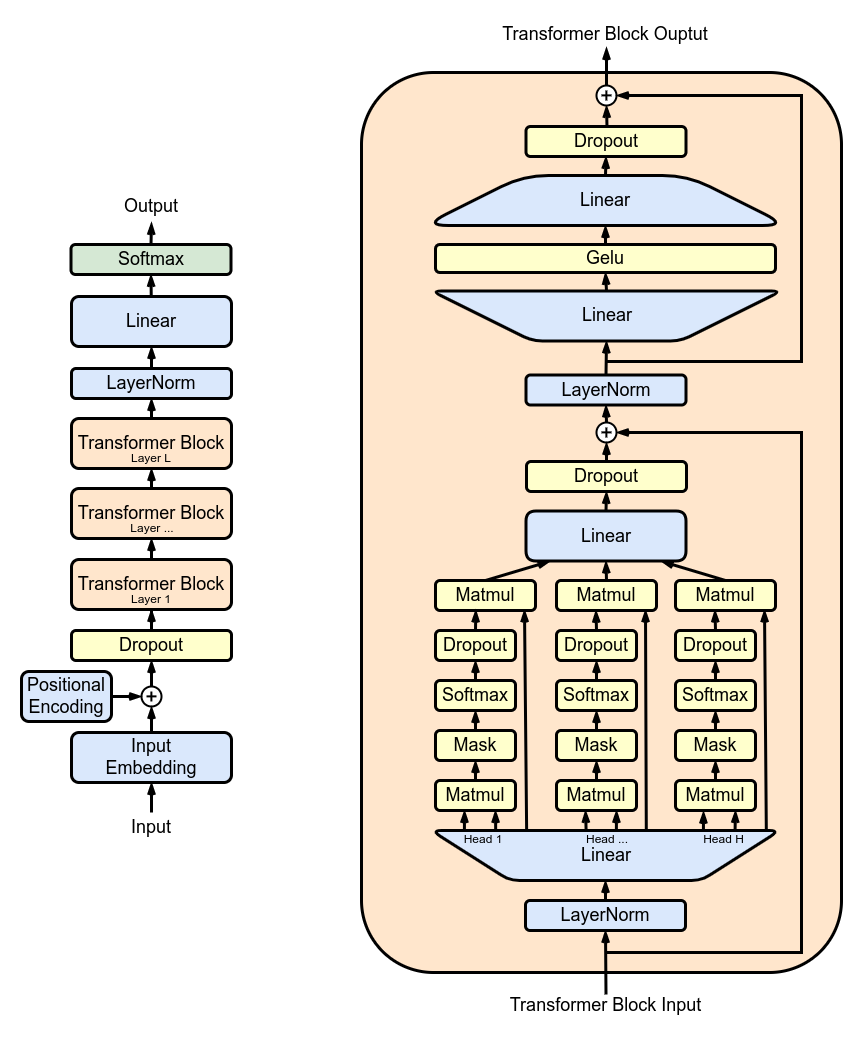
\includegraphics[width=0.55\textwidth]{obrazky/Full_GPT_architecture.png}
    \caption{Architektúra GPT. Prebrané z~\cite{gptarchitecture}.}
    \label{fig:GPT-architecture}
\end{figure}

\section{Generovanie zdrojového kódu}\label{sec:code_gen}

V~oblasti informačných technológií predstavuje generovanie zdrojového kódu spojenie ľudskej kreativity s~presnosťou a automatizáciou, ktorú poskytujú stroje. Proces transformácie myšlienok vyjadrených v~prirodzenom jazyku do presných, vykonateľných programovacích inštrukcií otvára nové možnosti vo vývoji softvéru. 

Schopnosť generovať kód možno chápať ako druh generovania prirodzeného jazyka. Tento proces možno konkrétne popísať ako preklad z~prirodzeného jazyka do programovacieho jazyka (Natural Language\,-\,Programming Language, NL\,-\,PL) a naopak. Generovanie kódu, ako forma prekladu, nie je iba jednoduché mapovanie slov medzi dvoma jazykmi; ide o~premostenie rozdielu v~logike, štruktúre a význame, ktoré tieto dva jazyky odlišujú.

Konceptuálny skok od prirodzeného jazyka k~jazyku programovania a naopak je zložitý, pretože oba jazyky slúžia veľmi odlišným účelom. Prirodzený jazyk je flexibilný, bohatý a umožňuje veľkú variabilitu. Naproti tomu programovací jazyk je definovaný svojou štruktúrou a predvídateľnosťou.

\noindent Podľa práce~\cite{ren2020codebleu} sú hlavné rozdiely medzi prirodzeným jazykom a programovacím jazykom nasledovné:
\begin{itemize}
    \item \textbf{Obmedzené kľúčové slová vs. milióny slov}: Na rozdiel od prirodzených jazykov s~veľkou slovnou zásobou, ktoré sa vyvíjali dlhú dobu a menili sa v~priebehu rokov, sú programovacie jazyky navrhnuté ľuďmi a používajú malý počet kľúčových slov. Tieto kľúčové slová sú pre programovacie jazyky kritické, definujú ich syntax a sémantiku, a preto by im mala byť venovaná zvýšená pozornosť.

    \item \textbf{Stromová štruktúra vs. sekvenčná štruktúra}: Prirodzené jazyky sú zvyčajne písané a čítané sekvenčne, zatiaľ čo programovacie jazyky sú reprezentované stromovou štruktúrou. Táto štruktúra je dôležitá pre správne vykonanie programu, a preto je dôležité, aby generovaný kód bol syntakticky správny.

    \item \textbf{Unikátne inštrukcie vs. nejednoznačná sémantika}: Prirodzené jazyky majú často nejednoznačnú a premennú sémantiku. Naproti tomu programovací jazyk vyžaduje štandardizáciu a systematickosť v~definícii inštrukcií. Každý výraz alebo príkaz v~programovacom jazyku má presne definovanú funkcionalitu, čo eliminuje nejednoznačnosť a zaisťuje, že program bude vykonaný tak, ako bol zamýšľaný. Tento prístup znižuje možnosť výkladových chýb, ktoré sú v~prirodzených jazykoch pomerne bežné v~dôsledku ich inherentnej nejednoznačnosti.
\end{itemize}

Pokiaľ ide o~výzvy a príležitosti, ktoré generovanie zdrojového kódu prináša, existujú rôzne aspekty, na ktoré sa treba sústrediť. Jedným z~hlavných aspektov je zlepšenie presnosti a účinnosti tohto procesu. Jazykové modely musia byť schopné pochopiť nielen textový opis funkcie alebo požiadavky, ale aj kontext, v~ktorom bude kód použitý. To vyžaduje pokročilé metódy spracovania prirodzeného jazyka a schopnosť analyzovať a interpretovať veľké množstvo dát.

\chapter{Trénovanie veľkých jazykových modelov}\label{chap:training}

Trénovanie jazykových modelov môže byť založené na rôznych prístupoch a zahŕňať niekoľko fáz, tak ako je vidieť na obrázku~\ref{fig:training}. Medzi prístupy učenia patrí učenie pod dohľadom (angl. supervised learning), učenie bez dohľadu (angl. unsupervised learning) a posilňované učenie (angl. reinforcement learning). Pri učení pod dohľadom model využíva označené dáta, kde každý vstup je priradený k~preddefinovanému výstupu. Učenie bez dohľadu pracuje s~neoznačenými dátami a model sa snaží nájsť štruktúru alebo vzory v~dátach bez vonkajších označení. Posilňované učenie, ktoré je často využívané pri veľkých konverzačných modeloch, umožňuje modelu učiť sa z~vlastných chýb prostredníctvom systému odmien a trestov. Model je pri tomto spôsobe odmeňovaný za správne reakcie a trestaný za chyby, čo ho motivuje k~neustálemu zlepšovaniu.

Trénovanie modelov, ktoré obsahujú veľké množstvo parametrov, vyžaduje rozsiahle dátové sady a významné výpočtové zdroje, najmä v~podobe výkonných grafických kariet. To predstavuje jednu z~hlavných výziev v~oblasti vývoja umelej inteligencie, keďže náklady na výpočtové zdroje môžu byť značné.

Techniky efektívneho ladenia parametrov (Parameter-Efficient Fine-Tuning, PEFT) poskytujú riešenie týchto výziev tým, že umožňujú trénovanie veľkých jazykových modelov s~menšími výpočtovými nárokmi. Tento prístup dosahuje úspory zmenšením počtu priamo trénovaných parametrov alebo aplikovaním techník, ako je kvantizácia váh modelu. V~tejto kapitole sa venujem technikám trénovania veľkých jazykových modelov. Rozoberiem jemné ladenie a ďalšie metódy, ktoré umožňujú efektívne trénovanie modelov pri nižších výpočtových nárokoch.

\section{Predtrénovanie}

Modely, ako je \GPT{}, sú predtrénované na rozsiahlych sadách, ktoré zahŕňajú knihy, články a webové stránky, aby poskytli komplexný jazykový základ. Architektúra modelu, najmä mechanizmus samopozornosti, o~ktorom sa hovorilo v~sekcií~\ref{sec:self-attention}, umožňuje modelom zachytiť zložité vzory v~jazyku, čo umožňuje vytvárať presné a sémanticky bohaté reprezentácie textu.

\begin{figure}[H]
    \centering
    \includesvg[width=0.8\textwidth]{obrazky/Training.svg}
    \caption{Trénovanie modelu prebieha v~niekoľkých fázach. Obvykle začína predtrénovanie, nasledované jemným ladením a posilňovaným učením modelu. Vo fázach sú potrebné rôzne dáta, z~ktorým sa model učí.}
    \label{fig:training}
\end{figure}

\subsection*{Príčinné modelovanie jazyka}

Modely založené na architektúre dekodéru, ako \GPT{} alebo \LLAMA{}, používajú metódu autoregresie. Inými slovami, model predikuje ďalší token v~sekvencii na základe predchádzajúcich stavov, smerov zľava-doprava, a porovnáva ho s~referenčným riešením.

\subsection*{Maskované modelovanie jazyka}

Táto techniku bola použitá pri trénovaní kodér modelu \BERT{}~\cite{devlin2019bert}. Jej podstatou je náhodné maskovanie časti vstupu a následné generovanie tokenov. Za správne riešenie sú považované maskované časti. Tento prístup umožňuje modelu učiť sa kontextovú reprezentáciu slov a ich vzťahy v~sekvencii.

\subsection*{Vyplňovanie na základe okolia}

Autoregresívne dekodér modely, ktoré sú v~súčasnosti prevažujúcou technológiou v~modelovaní jazyka pre generovanie ďalšieho slova v~sekvencii, pracujú výlučne s~kontextom na ľavej strane (prefix). Úloha vyplňovania na základe okolia (Fill in the Middle, FIM)~\cite{fedus2018maskgan,yang2020xlnet,bavarian2022efficient} predstavuje špecifický druh modelovania jazyka, ktorý umožňuje dekodér modelom generovať sekvencie so zreteľom na kontext umiestnený na oboch stranách. Prístup FIM dovoľuje modelom efektívne využívať informácie z~oboch strán sekvencie tým, že vykonáva permutáciu podsekvencií, čím model dostane informácie z~okolia miesta a následne generuje strednú časť. Umožňuje tak jazykovým modelom pre generovanie kódu napríklad predikovať názvy funkcií na základe kontextu v~tele funkcie, písať komentáre na základe kódu alebo doplniť chýbajúce časti kódu na základe kontextu v~okolí.

\section{Ladenie}

Po predtrénovaní sú modely ladené na menšej úlohe, špecifickej kolekcií dát. Táto fáza prispôsobuje široko naučené vzorce špecifickým aplikáciám. Ladenie vyžaduje označené údaje a prebieha pod dohľadom (supervised learning), čo znamená, že vstupný text je spojený so správnymi výstupmi alebo označeniami klasifikácie. Počas tejto fázy dochádza ku gradientovým úpravám všetkých váh modelu za účelom minimalizácie rozdielu medzi predpoveďami a skutočnými označeniami, čím sa zlepší presnosť na špecifickú úlohu.

Ladenie umožňuje prispôsobenie všeobecne predtrénovaného modelu širokej škále aplikácií, využívajúc komplexné porozumenie získané počas predtrénovania a aplikujúc ho na konkrétne úlohy. Tento prístup výrazne znižuje čas a zdroje potrebné na vývoj vysoko výkonných modelov pre špecifické aplikácie.

\subsection{Efektívne ladenie parametrov}
Jazykové modeli sa v~čase zlepšujú, ale to prichádza aj so stále sa zväčšujúcim počtom trénovateľných váh, ktoré sa v~súčasnosti pohybujú v~desiatkach až stovkách miliárd, GPT-3 má 175 miliard parametrov~\cite{brown2020language}, PaLM model až 540 miliárd~\cite{chowdhery2022palm}. Úplné ladenie váh predtrénovaných modelov sa so zväčšujúcimi modelmi stáva čoraz náročnejším. Z~tohto dôvodu bol vyvinutý koncept PEFT, ktorý umožňuje efektívnejšie využitie počtu parametrov. Táto technika sa sústreďuje na optimalizáciu malého počtu kľúčových parametrov namiesto upravovania celého modelu, čím sa výrazne znižujú nároky na výpočtové zdroje a čas potrebný pre ladenie.

PEFT využíva metódy ako napríklad selektívne trénovanie iba určitých vrstiev modelu alebo zavedenie nových, špecificky nastaviteľných parametrov, ktoré sa dajú efektívnejšie trénovať v~kontexte konkrétnej úlohy. Nasadenie techniky PEFT tak prináša značné výhody vo flexibilite, efektivite a škálovateľnosti ladenia jazykových modelov, čo je kľúčové pre ich široké využitie v~rôznych aplikáciách a pri rýchlo meniacich sa požiadavkách.

\subsection{Kvantizácia váh modelu}

Kvantizácia váh modelu~\cite{rokh2022modelquantization} je sofistikovaný proces, ktorý umožňuje preklenúť medzeru medzi presnosťou spojitého priestoru a praktickou potrebou kompaktnej reprezentácie. Prostredníctvom kvantizácie je možné váhy neurónových sietí, pôvodne reprezentované s~vysokou presnosťou v~spojitom rozsahu, transformovať na hodnoty s~nižšou bitovou hĺbkou reprezentované v~diskrétnom priestore. Tento proces sa vykonáva aplikáciou kvantizačnej funkcie, ktorá priradí každej pôvodnej hodnote najbližšiu hodnotu z~preddefinovaného súboru kvantizačných úrovní. Napríklad pri kvantizácií váh modelu z~pôvodnej reprezentácie 32-bitového čísla s~pohyblivou desatinnou čiarkou na 8-bitové celé čísla je prechod z~rozsahu $[-3.4\times 10^{38}, 3.4\times 10^{38}]$ na rozsah $[-128, 127]$. Tento proces umožňuje zmenšiť veľkosť modelu a zvýšiť efektivitu pri výpočtoch, ale za cenu straty presnosti.

V~kontexte trénovania jazykových modelov sa kvantizácia využíva na zmenšenie počtu parametrov modelu, čím sa znižujú výpočtové a priestorové nároky potrebné na trénovanie a nasadenie modelu. Tento prístup umožňuje efektívne trénovanie veľkých modelov na zariadeniach s~obmedzenými výpočtovými zdrojmi, čo je kľúčové pre ich nasadenie v~reálnom svete.


\subsection{Adaptácia nízkorozmerných reprezentácií}

Adaptácia nízkorozmerných reprezentácií (Low-Rank Adaptation, LoRA) čerpá inšpiráciu z~prác, ktoré ukázali, že modely s~nadmerným počtom parametrov (over-parametrized models) v~skutočnosti existujú v~priestore s~nízkou vnútornou dimenziou. To znamená, že aj keď modely majú veľký počet parametrov, ich efektívne správanie a schopnosť generalizácie môže byť opísané podstatne menším počtom relevantných dimenzií~\cite{hu2021lora}.

Na základe tohto pozorovania autori formulovali hypotézu, že zmeny vo~váhach modelu počas jeho adaptácie (napríklad pri ladení na špecifickú úlohu) majú nízky vnútorný rozmer alebo \uv{intrinsic rank}. Inak povedané, predpokladali, že aj keď sa počas adaptácie modelu upravuje veľký počet váh, skutočná efektívna zmena, ktorá sa deje v~modeli, môže byť opísaná menším počtom kľúčových dimenzií alebo parametrov.

Ako je znázornené na obrázku~\ref{fig:lora}, predtrénovanú váhová matica $(W_0 \in \mathbb{R}^{d \cdot k})$ sa aktualizuje pomocou nízkorozmernej dekompozície $W_0 + \Delta W = W_0 + BA$, kde $B \in \mathbb{R}^{d \cdot r}$, $A \in \mathbb{R}^{r \cdot k}$, a hodnosť $r$ je menšia ako $min(d, k)$. Týmto prístupom sa udržiavajú pôvodné váhy $W_0$ fixné, zatiaľ čo $A$ a $B$ sú trénovateľné. To umožňuje modelu adaptovať sa na nové úlohy bez potreby zásadných zmien v~jeho štruktúre.

Pri tomto procese $W_0$ a $\Delta W = BA$ pracujú na rovnakom vstupe a ich výsledky sú sčítané podľa súradníc. Takto upravený dopredný prechod pre $h = W_0x$ poskytuje výsledok: $$h = W_0x + \Delta W x = W_0x + BAx$$ 

\begin{figure}
    \centering
    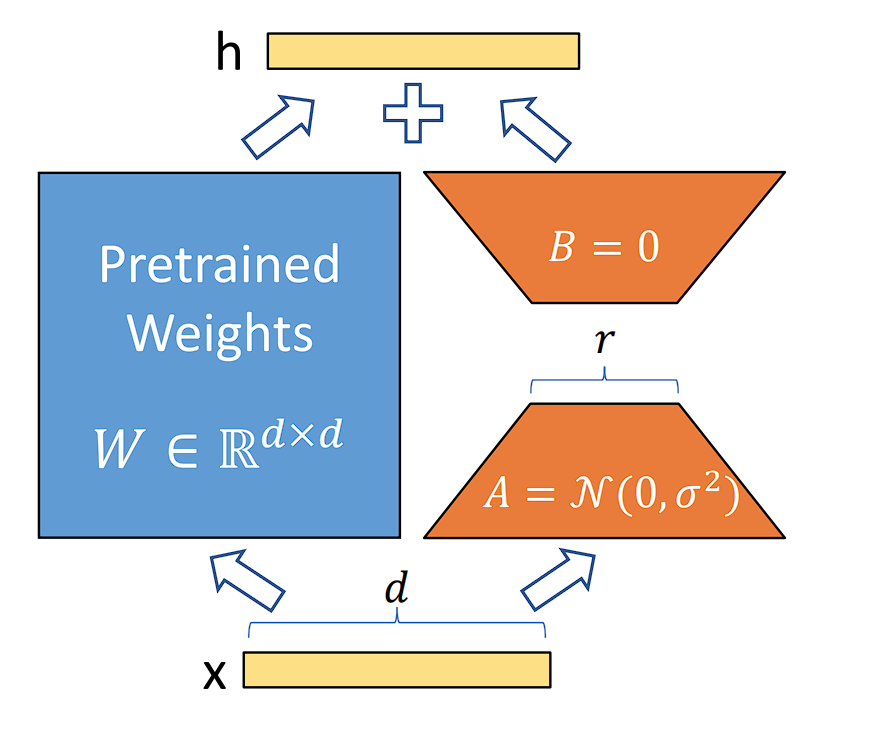
\includegraphics[width=0.4\textwidth]{obrazky/LoRA.png}
    \caption{Váhy matice $A$ sú inicializované náhodne Gaussovým rozdelením. Matica $B$ je inicializovaná nulami, takže matica $\Delta W = BA$ je na začiatku tréningu nulová. Počas trénovania sa $A$ a $B$ upravujú pomocou gradientných metód, čím sa model adaptuje na špecifickú úlohu. Prebrané z~\cite{hu2021lora}.}
    \label{fig:lora}
\end{figure}

\subsection{QLoRA}

Technika QLoRA (Quantized Low-Rank Adaptation)~\cite{dettmers2023qlora} kombinuje kvantizáciu váh modelu s~LoRA, čím umožňuje efektívne trénovanie rozsiahlych modelov. Najprv sa váhy modelu kvantizujú na nižšiu bitovú hĺbku, po ktorej sa pridajú nízkorozmerné dekompozície $A$ a $B$. Váhy v~maticiach $A$ a~$B$ sú v~16-bitovej presnosti. Tieto reprezentácie sú následne trénované pomocou spätného šírenia chýb cez kvantizované váhy modelu. Autori práce predstavili stránkovaný optimalizátor (Paged Optimizer), ktorý využíva stránkovanie CPU a aktivuje sa, keď sa vyčerpá pamäť GPU. Keď sa tak stane, pamäť sa presúva stránka po stránke z~GPU na CPU, čo zabezpečuje efektívnu správu pamäťových požiadavkov. Týmto spôsobom sa zmierni vplyv rýchlych pamäťových nárastov pri ukladaní kontrolných bodov gradientov (angl. gradient checkpointing), ktoré sa vyskytujú pri spracovaní dávky s~väčšou dĺžkou sekvencie.

\begin{figure}
    \centering
    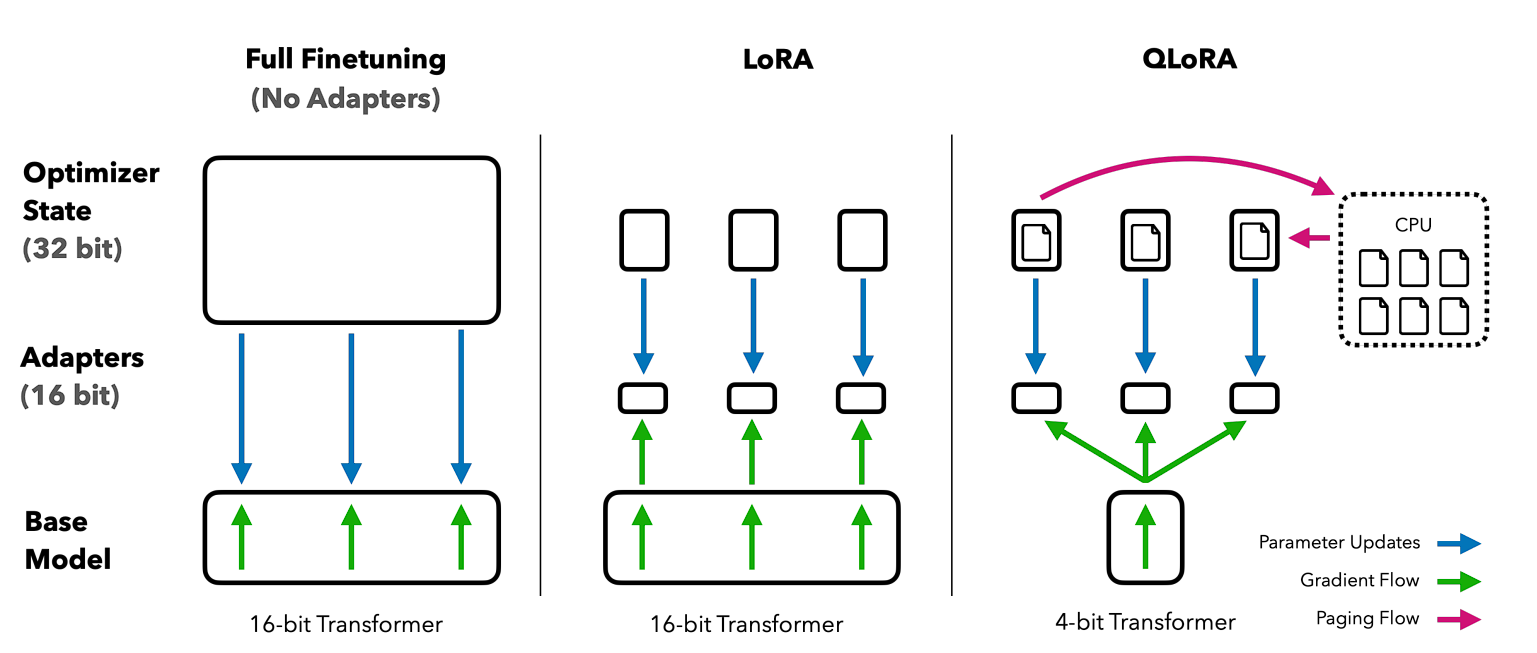
\includegraphics[width=0.8\textwidth]{obrazky/QLoRA.png}
    \caption{Porovnanie prístupu plného ladenia všetkých váh, techniky LoRA a techniky QLoRA. Prebrané z~\cite{dettmers2023qlora}.}
    \label{fig:qlora}
\end{figure}

\section{Evaluačné metriky}

Pri vývoji modelov pre generovanie kódu je kľúčovým aspektom vývoja ich evaluácia. Evaluácia modelov v~tejto oblasti sa líši od tradičného hodnotenia modelov strojového učenia. Kód, na rozdiel od prirodzeného jazyka, vyžaduje syntaktickú presnosť, sémantickú správnosť a funkčnú vykonateľnosť. Bežné metriky z~oblasti prirodzeného jazyka zanedbávajú dôležité sémantické a syntaktické vlastnosti kódu alebo podceňujú syntakticky odlišné výstupy s~rovnakou sémantickou logikou.

V~nasledujúcich sekciách predstavím 3 rôzne prístupy pre evaluáciu modelov pre generovanie kódu. Prvý prístup predstavujú metriky, ktoré boli pôvodne navrhnuté pre hodnotenie strojového prekladu, druhý prístup predstavuje metriky, ktoré boli navrhnuté špecificky pre hodnotenie generovania kódu. Tieto dva prístupy porovnávajú generovaný kód s~referenčným kódom, prípadne viacerými variantami, a hodnotia syntaktickú a sémantickú podobnosť medzi nimi. Tretí prístup predstavujú metriky založené na vykonávaní generovaného kódu a hodnotení jeho správnosti sadou preddefinovaných testov.

\subsection{BLEU}
BLEU (Bilingual Evaluation Understudy)~\cite{papinenibleu2002} predstavuje algoritmus pre evaluáciu kvality strojovo preložených textov. Kritériom kvality je presnosť (angl. precision\footnote{V~slovenčine je termín \uv{presnosť} používaný aj pre anglický termín \uv{accuracy}, čo môže viesť k~nejasnostiam. Pre \uv{accuracy} je vhodnejší preklad \uv{správnosť}.}), alebo miera zhody, medzi výstupom strojového prekladu a prekladom vykonaným človekom.

Myšlienka BLEU je založená na výpočte presnosti n-gramov\footnote{N-gram je označenie pre skupinu po sebe idúcich slov. Teda napríklad unigramy budú slová samotné a bigramy dvojice za sebou idúcich slov.}. Rovnica~\ref{eq:precision} definuje presnosť, ktorá sa počíta ako podiel počtu zhodných slov v~preklade a referenčnom preklade (True Positive, TP) a počtu všetkých slov v~strojovom preklade, ktoré ale môžu obsahovať aj slová nevyskytujúce sa v~referenčnom preklade (False Positive, FP).

\begin{equation}\label{eq:precision}
Precision = \frac{TP}{TP+FP}
\end{equation}

Tu treba poznamenať, že napríklad pre strojový preklad \texttt{sum sum sum sum sum} a referenčný preklad \texttt{sum = a + b}, by bol rovný $1$. Tento prístup je zjavne nedostačujúci, a tak BLEU zavádza modifikovanú presnosť n-gramov. Modifikácie je transformovaná do obmedzenia počtu možných zhôd daného slova podľa toho, koľkokrát sa vyskytuje v~referenčnom preklade. Inými slovami, ak sa slovo \texttt{sum} vyskytuje v~referenčnom preklade iba raz, tak počet zhôd tohto slova môže byť najviac $1$. Pre predošlý príklad je výsledok modifikovanej presnosť unigramov rovný $1/5$. Skóre BLEU je váženým súčtom týchto modifikovaných zhôd pre n-gramy. Dlhšie n-gramy sú zvyčajne presnejšie, pretože sú menej pravdepodobné, že sa vyskytnú náhodne. Preto BLEU zavádza váhy pre n-gramy, ktoré zohľadňujú ich dĺžku.

Dlhšie vygenerované sekvencie ako referenčné sú z~podstaty výpočtu penalizované. To neplatí pre sekvencie, ktoré sú kratšie ako referenčné. Preto BLEU závadza penalizáciu krátkych sekvencií (brevity penalty). Výsledné skóre BLEU je definovane v~rovnici~\ref{eq:bleu}.

\begin{equation}\label{eq:bleu}
    BLEU = BP\cdot\exp\left(\sum_{n=1}^{N}w_n\log p_n\right),
\end{equation}
\noindent kde $BP$ je brevity penalty, $w_n$ je váha n-gramu, $p_n$ je modifikovaná presnosť n-gramu a $N$ je maximálna dĺžka n-gramu.

\subsection{CodeBLEU}

Tak ako bolo spomenuté v~podkapitole~\ref{sec:code_gen}, medzi prirodzenými jazykmi a programovacími jazykmi existujú zásadné rozdiely, ktoré znamenajú, že metriky navrhnuté pre hodnotenie kvality prekladu medzi prirodzenými jazykmi nemusia byť vhodné pre hodnotenie generovania kódu. Preto boli navrhnuté metriky, ktoré sú špecificky prispôsobené pre hodnotenie generovania kódu. Jednou z~týchto metrík je CodeBLEU~\cite{ren2020codebleu}, ktorá je založená na metrike BLEU, ale bola upravená tak, aby zohľadňovala špecifiká programovacích jazykov.

\noindent Metrika CodeBLEU pridáva do výpočtu tri nové faktory a to:
\begin{enumerate}
    \item výpočet presnosti n-gramov s~vyššími váhami pre kľúčové slová programovacieho jazyka,

    \item abstraktné syntaktické stromy porovnávaných kódov,

    \item Orientované grafy pre reprezentáciu toku hodnôt premenných v~kóde.
\end{enumerate}

\noindent Výsledné skóre je váženým súčtom týchto faktorov a pôvodného skóre BLEU :
\begin{equation}\label{eq:codebleu}
    CodeBLEU = \alpha\cdot BLEU + \beta\cdot BLEU_{weight} + \gamma\cdot Match_{ast} + \delta\cdot Match_{df}
\end{equation}

\subsection{ROUGE}
ROUGE (Recall-Oriented Understudy for Gisting Evaluation)~\cite{lin2004rouge} je metrika používaná na evaluáciu automatického generovania zhrnutí alebo iných textových úloh, kde je dôležitá miera zhody medzi generovaným výstupom a referenčným textom. Na rozdiel od BLEU, ktoré je zamerané na presnosť, ROUGE posudzuje n-gramovú zhodu z~hľadiska úplnosti (angl. recall), teda podiel počtu zhodných slov v~generovanom texte a počtu slov v~referenčnom texte.

ROUGE je sada viacerých variant, ako napríklad ROUGE-N (n-gramová úplnosť), ROUGE-L (najdlhšia spoločná sekvencia), a ROUGE-S (zhoda založená na preskakovaní n-gramov). Tieto metriky umožňujú posúdiť text z~rôznych perspektív, čo je dôležité pri komplexných úlohách, ako je zhrnutie textu, kde môže byť mnoho platných formulácií.

\begin{equation}\label{eq:rouge}
ROUGE-N = \frac{\sum_{s \in {Reference}} \sum_{gram_n \in s} Count_{match}(gram_n)}{\sum_{s \in {Reference}} \sum_{gram_n \in s} Count(gram_n)}
\end{equation}

\subsection{ChrF}
ChrF (Character n-gram F-score)~\cite{popovic2015chrf} je metrika, ktorá hodnotí kvalitu prekladu alebo textového generovania na základe zhody znakových n-gramov medzi referenčným a generovaným textom. Na rozdiel od slovne orientovaných metrík, ako BLEU alebo ROUGE, chrF skúma text na úrovni znakov, čo umožňuje zachytiť jemnejšie nuansy jazyka, ako sú koncovky slov a morfologické štruktúry. Výpočet metriky chrF je založený na výpočte F-skóre, ktoré je váženým súčtom presnosti a úplnosti:

\begin{equation}\label{eq:chrf}
    ngrF_{\beta} = (1 + \beta^2) \cdot \frac{ngrP \cdot ngrR}{\beta^2 \cdot ngrP + ngrR},
\end{equation}

\noindent kde  $\beta$ je parameter, ktorý ovplyvňuje vzájomnú váhu presnosti a úplnosti, $ngrP$ je presnosť znakových n-gramov a $ngrR$ je úplnosť znakových n-gramov.

Verzia chrF{++}~\cite{popovic2017chrf}, ktorá je rozšírením pôvodnej metriky, zahrňuje do výpočtu okrem znakových n-gramov aj slovné unigramy a bigramy. Vďaka tomu chrF++ kombinuje výhody znakových a slovných metrík, čo umožňuje lepšiu koreláciu s~referenčným textom a presnejšie hodnotenie kvality generovaného textu. ChrF{++} vypočítame ako aritmetický priemer F-skóre pre znakové n-gramy a slovné k-gramy.

\subsection{Pass@k}

Metrika pass@k~\cite{kulal2019spoc} sa používa pre hodnotenie funkčnej správnosti kódu vygenerovaného modelom. Základná myšlienka spočíva v~nedostatku metrík založených na porovnávaní s~referenčným výstupom, ktoré nemôžu zachytiť komplexný priestor ekvivalentných riešení a navyše majú problém zachytiť sémantické špecifiká kódu. Preto sa pass@k zameriava na vykonanie generovaného kódu a vyhodnotenie jeho správnosti pomocou sady vopred definovaných testovacích príkladov. Inšpiráciu nachádza v~testovaním riadenom vývoji softvéru (Test-Driven Development, TDD), ktoré je štandardnou praxou v~softvérovom inžinierstve. Metrika sa používa ako hodnotiace kritérium toho, či je kód správne implementovaný. Práca~\cite{chen2021evaluating} definuje pass@k ako:
$$
pass@k := E\left[1 - \left(\frac{\binom{n-c}{k}}{\binom{n}{k}}\right)\right],
$$

\noindent kde $k$ je počet zvolených riešení z~$n \geq k$ vygenerovaných vzoriek pre daný príklad. Premenná $c \leq n$ je počet vzoriek, ktoré úspešne prešli testovaním.

Zjavnou nevýhodou tejto metriky je, že vyžaduje existenciu sady testovacích príkladov pre konkrétnu úlohu. Tieto príklady musia byť navyše vysokej kvality a musia pokrývať širokú škálu možných riešení. Vykonávanie strojovo generované kódu môže predstavovať bezpečnostné riziká. Je preto potrebné mať k~dispozícii izolované testovacie prostredie, ktoré umožní bezpečné vykonávanie kódu. V~oblasti programovania vstavaných systémov a mikrokontrolérov je toto obzvlášť dôležité, pretože chyby v~kóde môžu mať vážne následky na fyzické zariadenie. Preto je v~tejto oblasti na zváženie použitie nástrojov na emuláciu hardvéru.

\subsubsection{Dátová sada HumanEval}

Zlatý štandard v~oblasti funkčného testovania modelov je dátová sada HumanEval~\cite{chen2021evaluating}. HumanEval je ručne vytvorená dátová sada, ktorá je špeciálne navrhnutá na evaluáciu schopností generovania kódu umelou inteligenciou v~jazyku Python a obsahuje 164 príkladov. Úlohy v~sade HumanEval sú formulované ako funkcie, ktoré vyžadujú naprogramovanie správneho riešenia na základe špecifikovaných požiadaviek. Každá úloha obsahuje textuálny popis, signatúru, telo funkcie a súbor testovacích prípadov, ktoré overujú funkčnosť riešenia. Tieto testy zahŕňajú vstupy a očakávané výstupy, čím poskytujú objektívne meradlo úspešnosti riešenia.

\chapter{Prehľad súčasných riešení}\label{chap:survey}

V~tejto kapitole predstavím pokročilé modely pre generovanie zdrojového kódu a ich vlastnosti. Poviem, v~čom sa do seba odlišujú, a zhrniem výhody a nevýhody použitia daného modelu. V~súčasnosti prebieha vývoj veľkých jazykových modelov rýchlym tempom. Nové modely vychádzajú na mesačnej, ak nie na týždennej báze a je náročné sledovať vývoj v~tejto oblasti. Preto vyberám iba niektoré  modely, ktoré sú zaujímavé z~hľadiska práce. Pred tým, ako sa dostanem k~samotným modelom, je potrebné si povedať niečo o~dátových sádách, ktoré sú používané na trénovanie týchto modelov, a to predovšetkým v~oblasti vstavaných systémov a mikrokontrolérov.

\section{Dátové sady pre generovanie kódu}

V~oblasti generovania kódu existuje množstvo dátových sád, ktoré sú špeciálne navrhnuté na trénovanie modelov pre generovanie kódu. Tieto dátové sady zahŕňajú rôzne typy kódov, ako sú napríklad kódy z~webových stránok, kódy z~verejných repozitárov alebo z~programovacích súťaží. V~súčasnosti existuje množstvo verejne dostupných dátových sád, ktoré sú špeciálne zamerané na generovanie kódu v~jazykoch ako Python, Java, C++ alebo JavaScript.

V~oblasti programovania vstavaných systémov a mikrokontrolérov som pri hľadaní narazil iba na jednu dátovú sadu~\cite{9590539}. Táto dátová dada bohužiaľ nie je dostupná pre širokú verejnosť. Navyše je pomerne malá (1000 vzoriek) a nie je zameraná na generovanie kódu, ale na jeho klasifikáciu. Myslím si, že výskum v~danej problematike má zmysel. Je preto vhodné vytvoriť nové dátové sady zamerané na generovanie kódu pre vstavané systémy a mikrokontroléry. Štruktúra a proces tvorby vzoriek spomínanej dátovej sady poskytuje vhodný príklad potenciálnej stavby vzoriek novej dátovej sady.

\section{Prehľad modelov pre generovanie kódu}

\subsection{Codex}

\textsc{Codex}~\cite{chen2021evaluating} je séria modelov, ktoré vznikli ladením GPT-3 na rozsiahlej kolekcií dát kódu a textov prirodzeného jazyka. Dátová sada pre trénovanie Codex modelov vznikla zozbieraním 54 miliónov verejne dostupných repozitárov na platforme GitHub a má celkovú veľkosť 159\,GB. Codex, presnejšie verzia \textsc{Codex 12B} s~dvanástimi miliardami parametrov, tvoril jadro nástroja GitHub Copilot. Je schopný generovať kód v~rôznych jazykoch, vrátane jazyka Python, JavaScript, Go, PHP, Ruby, Swift alebo TypeScript.

Značnou nevýhodou je jeho uzavretosť a nedostupnosť váh. To nedovoľuje trénovať model na vlastných dátach, a tým prispôsobiť ho na konkrétnu úlohu. Na druhej strane tak, ako je možno vidieť v~tabuľke~\ref{tab:humanevalscore}, \textsc{Codex 12B} dosahuje vysoké skóre a je schopný generovať kód na základe krátkych popisov a požiadaviek. Môže tak slúžiť ako referenčný model pri vývoji iných modelov.

\begin{table}[!ht]
    \centering
    \begin{tabular}{r | c c c}
        Model & pass@1 & pass@10 & pass@100 \\ \hline
        \textsc{Codex 12B} & 28,81\,\% & 46,81\,\% & 72,31\,\% \\
        \CL{} & 34,8\,\% & 64,3\,\% & 88,1\,\%\\ 
        \SC{} & 15,17\,\% & \textemdash & \textemdash
    \end{tabular}
    \caption{Reportované pass@k skóre jednotlivých modelov na sade príkladov HumanEval.}
    \label{tab:humanevalscore}
\end{table}


\subsection{CodeLLaMA}\label{sec:codellama}

\CL{} je súčasťou širšej rodiny voľne prístupných veľkých jazykových modelov pre generovanie a doplňovanie kódu \textsc{Code LLaMA}~\cite{roziere2024code}. Označenie \textsc{7B} v~názve značí počet váh. Konkrétne sa skladá z~32 dekodér blokov spolu s~takmer siedmimi miliardami parametrov, čo ho stavia do pozície modelu so značným výpočtovým výkonom a inteligenciou. Označenie \textsc{Instruct} hovorí, že tento model bol ladený tak, aby odpovede lepšie zodpovedali zadaným pokynom, a to posilňovaným učením s~využitím špeciálnej dátovej sady.

Modely \textsc{Code Llama} vznikli trénovaním modelov \textsc{Llama 2}~\cite{touvron2023llama}, ktoré sú pôvodne určené pre modelovanie prirodzeného jazyka. Tieto modely následne ďalej trénovali na sade veľkého množstva zdrojových súborov a vzoriek prirodzeného jazyka súvisiacich s~kódom. Čo sa týka vzoriek zameraných na prirodzený jazyk, tak aj tieto súvisia s~kódom a ide napríklad o~príspevky na diskusných fórach, ktoré diskutujú rôzne programovacie problémy, ich riešenia, a obsahujú úryvky kódu. Model, ktorý som si zvolil, bol navyše ladený na troch dátových sadách s~celkovom veľkosťou 5 miliard tokenov, z~ktorých nás zaujímajú hlavne tieto:
\begin{enumerate}
        \item Kolekcia dát zameraná na užitočnosť a bezpečnosť, predstavená v~práci~\cite{touvron2023llama} -- približuje formát a štruktúru odpovede tak, aby bola bezpečná a obsahovala čo najviac užitočných informácií.
        \item Samoinštruovaná sada -- Približne 14\,000 trojíc (zadanie, testy a riešenie), zozbierané s~využitím modelov \textsc{Llama~2~70B} (generovanie zadania programovacieho problému) a \textsc{Code Llama 7B} (generovanie testov a správnych riešení problémov). Je zameraná na generovanie kódu na základe zadaného problému a testov, ktoré by mali byť splnené. Ide o~samoinštruovanú kolekciu, ktorá vznikla dopytovaním iných modelov namiesto použitia anotácie ľudí. Konkrétna sada je zaujímavá z~hľadiska interpretovateľnosti. Výsledky generovania testov a riešení poskytujú informácie pre analýzu schopností modelov. Na druhej strane, táto kolekcia dát môže obsahovať chyby, ktoré boli prenesené z~dotazovaných modelov.
\end{enumerate}

\newpage
\subsection{StarcoderBase}~\label{sec:starcoder}

\noindent\textsc{StarCoderBase}~\cite{li2023starcoder} je séria modelov predtrénovaných na podmnožine rozsiahlej kolekcie dát \textsc{The Stack (v\,1.2)}, ktorá obsahovala 1 bilión tokenov a kódy v~80 programovacích jazykoch. Tieto modely s~veľkosťou od 1 do 15,5 miliardy parametrov využívajú upravenú Multi-Head pozornosť, nazvanú Multi-Query pozornosť~\cite{shazeer2019fast} a kontextové okno viac ako 8\,tisíc tokenov.

Veľkou výhodou je ich rýchlosť inferencie, dosiahnutá použitím Multi-Query pozornosti (MQA), kde sa využívajú rovnaké matice $K$ a $V$ pre všetky paralelne pracujúce hlavy pozornosti, čo zrýchľuje inferenciu. Sú vhodné pre použitie v~reálnom čase, kde je dôležitá rýchlosť generovania kódu, a majú schopnosť generovať kód na základe kontextu, čo je užitočné pri nasadení vo vývojových prostrediach.

Nevýhodou je ich menšia veľkosť, čo môže ovplyvniť kvalitu generovaného kódu. Na rozdiel od modelov \textsc{Code Llama} nie sú ladené na inštruované odpovedanie, ale sú zamerané na rýchle generovanie kódu v~kontexte.

\subsection{DeepSeek-Coder}~\label{sec:deepseekcoder}

\noindent\DSC{}~\cite{guo2024deepseekcoder} je séria modelov s~veľkosťou od 1,3 do 33 miliárd parametrov. Modely boli predtrénované na 2 biliónoch tokenov z~87 programovacích jazykov. Využívajú prístup FIM s~kontextovým oknom 16K na zlepšenie generovania a dopĺňania kódu na úrovni projektu. Hlavnou prednosťou modelov \DSC{} je vysoký výkon a schopnosť prekonať aj existujúce uzavreté modely ako \textsc{Codex} alebo \textsc{GPT-3.5-Turbo}.

\DSC{} sú modely s~dekodér transformer architektúrou postavené na rovnakom základe ako \textsc{DeepSeek LLM}~\cite{deepseekai2024deepseek}. Využívajú \textsc{SwiGLU} aktivačnú funkciu, a najväčší model implementuje Grouped-Query pozornosť (GQA). GQA je ďalší typ MHA, ktorá rozdeľuje matice váh $W_Q$ do skupín tak, že skupina zdieľa jednu maticu $W_K$ a $W_V$. Tento prístup syntetizuje prednosti MHA a MQA, čím dosahuje vyššiu výpočtovú rýchlosť v~porovnaní s~MHA a zároveň prekonáva MQA v~kvalitatívnom hodnotení výstupov~\cite{ainslie2023gqa}.

\begin{figure}[!ht]
    \centering
    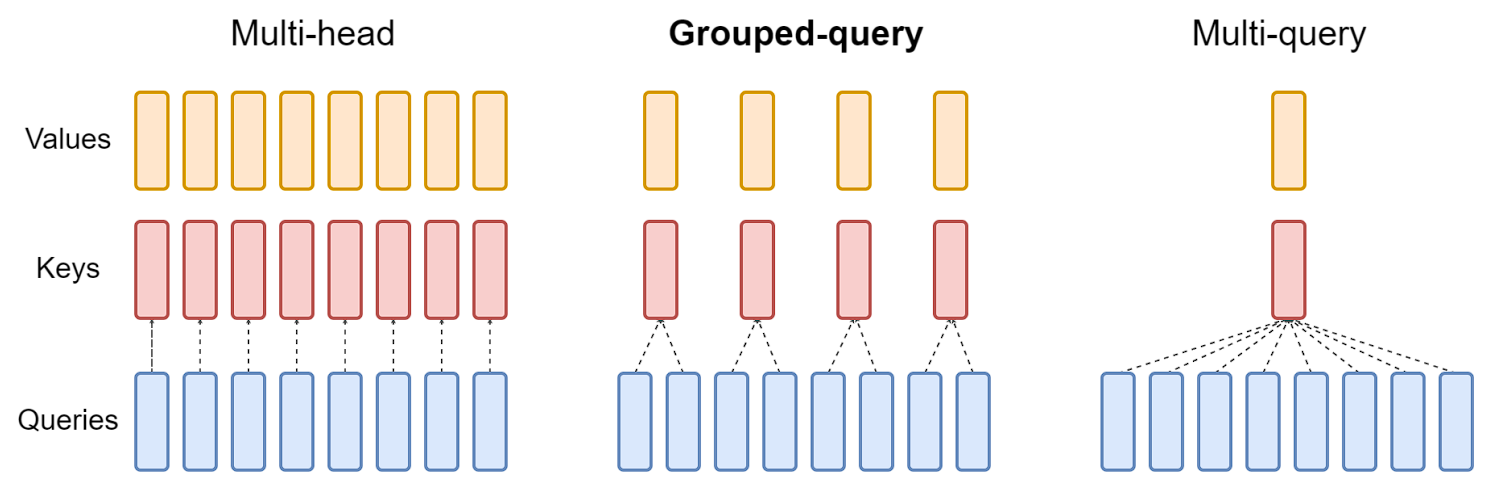
\includegraphics[width=0.8\textwidth]{obrazky/GQA.png}
    \caption{Prehľad metód pozornosti. MHA obsahuje rovnaký počet matíc $Q$, $K$ a $V$. GQA zdieľa jednu maticu $K$ a $V$ pre skupinu matíc $Q$, zatiaľ čo MQA zdieľa jedinú maticu $K$ a $V$ pre všetky $Q$. Prebrané z~\cite{ainslie2023gqa}.}
    \label{fig:mha-mqa-gqa}
\end{figure}



\chapter{Návrh a implementácia}\label{chap:implementation}

\begin{figure}[!ht]
    \centering
    \includesvg[width=0.5\textwidth]{obrazky/implementation.svg}
    \caption{Schéma návrhu riešenia práce.}
    \label{fig:implementation}
\end{figure}

V~tejto kapitole sa venujem popisu procesu tvorby dátovej sady z~existujúcich zdrojových súborov, následnému ladeniu predtrénovaných modelov na tejto dátovej sade a evaluácii vyvinutých modelov. Sekcia \ref{sec:dataset} poskytuje detailný popis metodiky vytvárania dátovej sady. V~sekcii~\ref{sec:dataset-analysis} následne na novej dátovej sade vykonávam stručnú analýzu niektorých jej vlastností. V~sekcií \ref{sec:finetuning} sa zaoberám kvantizáciou a trénovaním rozsiahlejšieho modelu \CL{} a trénovaním kompaktnejšieho \SC{} na vytvorenej dátovej sade. V~záverečnej sekcii \ref{sec:evaluation} je predstavená evaluácia modelov na súbore testovacích príkladov.

\section{Dátová sada}\label{sec:dataset}

Na zostavenie dátovej sady som využil zdrojové súbory z~platformy GitHub. Táto platforma umožňuje ukladať a spravovať rôzne súbory, ako sú predovšetkým zdrojové kódy, a umožňuje ich verejné zdieľanie s~ostatnými užívateľmi. Zdrojové súbory sú uložené v~gitových repozitároch, ktoré poskytujú priestor pre ukladanie súborov a zaznamenávanie histórie zmien v~projektoch. Pre účely práce som sa zameriaval na zdrojové súbory napísané v~jazykoch C++ alebo C, pretože tieto jazyky sú najčastejšie používané v~oblasti programovania vstavaných systémov a mikrokontrolérov.

\begin{figure}[!ht]
    \centering
        \includesvg[width=0.9\textwidth]{obrazky/dataset_prep.svg}
    \caption{Proces tvorby dátovej sady.}
    \label{fig:datset-prep}
\end{figure}

Výsledok krokov tvorby dátovej sady, ktoré popisujem nižšie, je dátová množina s~približne 50\,tisíc príkladmi. Dátovú sadu som rozdelil v~bežne používanom pomere $80:10:10$ na trénovaciu, validačnú a testovaciu podmnožinu. Každá vzorka obsahuje zadanie (textový popis a signatúra funkcie), a referenčné riešenie (vnútorný kód funkcie). Dátovú sadu som zverejnil a je voľne dostupná na platforme Hugging Face\footnote{\url{https://huggingface.co/datasets/xvadov01/cpp_emb_nl2pl}}. Povzbudzujem všetkých záujemcov o~danú oblasť generovania kódu, aby prispeli k~rozšíreniu dátovej sady alebo použili dáta na vytvorenie nových modelov.

\begin{figure}[!ht]
    \centering
    \includesvg[width=0.8\textwidth]{obrazky/example_structure.svg}
    \caption{Štruktúra vzorky dátovej sady.}
    \label{fig:data-example}
\end{figure}

\newpage

\subsection*{Zber zdrojových súborov}

Prvým krokom pri zbere dát bolo vyhľadávanie vhodných zdrojových súborov. Použil som dva prístupy:
\begin{enumerate}
    \item Vyhľadávanie projektov na základe témy, ktorú danému repozitáru pridelil jeho autor. V~tomto kroku som vyhľadával repozitáre s~témou \textsc{firmware}, \textsc{microcontroller} a \textsc{embedded-systems}. Z~každej témy bolo zvolených 50 repozitárov na základe kritéria udelených hviezd\footnote{Hviedzy udeľujú užívatelia. Počet hviezd, ktoré repozitár získal, je dobrým ukazovateľom užitočnosti a popularity. Vysoký počet hviezd naznačuje, že daný repozitár je v~komunite uznávaný.}.
    \item Vyhľadávanie na základe kľúčových slov v~metadátach repozitáru (názov, obsah súboru README, popis, \dots). Zameral som sa na vyhľadávanie kľúčových slov \textsc{Cortex-M0, Cortex-M0+, Cortex-M1, Cortex-M3, Cortex-M4, Cortex-A, STM32, ESP32} a \textsc{ESP8266}.
\end{enumerate}

\subsection*{Filtrovanie súborov a predspracovanie zdrojového kódu}

Z~každého stiahnutého repozitára boli vybrané iba zdrojové súbory v~jazyku C/C++. Súbory, ktoré neobsahovali zdrojový kód, ako napríklad dokumentácia alebo konfiguračné súbory, boli z~repozitárov odstránené. Tiež boli odstránené všetky priečinky a súbory, ktorých názov obsahoval slovo \texttt{test}.

Štýl písania popisov funkcií v~jednotlivých repozitároch sa líši. Snahou bolo upraviť čo najviac komentárov tak, aby vyhovovali štýlu \textsc{Javadoc}. Tento štýl je štandardným spôsobom písania popisov funkcií v~jazykoch C/C++ a je podporovaný mnohými nástrojmi na generovanie dokumentácie. Často sa vyskytoval formát, ktorý uvádzal komentár znakmi \verb|/*\n|\footnote{Označením nového riadku zdôrazňujem, že ide o~viacriadkový komentár.}, ten bol nahradený tak, aby komentár začínal \verb|/**\n|.

\subsection*{Extrakcia funkcií}

Z~každého zdrojového súboru boli extrahované individuálne funkcie, pretože cieľom je trénovať model na funkciách, nie na celých súboroch. Pre extrahovanie jednotlivých funkcií s~ich popisom som využil nástroj Doxygen, respektíve syntaktický analyzátor (parser), ktorý Doxygen poskytuje. Tento parser umožňuje spracovanie zdrojového súboru a generovanie jeho reprezentácie vo formáte \textsc{XML}. Parser identifikuje v~zdrojovom súbore popisy funkcií, ktoré programátor napísal v~určitom formáte. Blok komentára je následne spracovaný parserom a z~neho je vygenerovaná \textsc{XML} reprezentácia, ktorá obsahuje informácie o~funkcii, ako sú jej názov, popis, parametre a návratová hodnota. Podobne sú identifikované aj bloky funkcií, ktoré sú následne extrahované priamo zo zdrojového súboru.
    
Syntaktický analyzátor Doxygen je schopný identifikovať popisy funkcií, ktoré sú napísané v~rôznych štýloch. Štandardným spôsobom písania popisov funkcií v~jazykoch C/C++ je štýl \textsc{JavaDoc}, ktorý je podporovaný mnohými nástrojmi na generovanie dokumentácie.

Použil som prepínač \textsc{JAVADOC\_BLOCK}, ktorý umožní, aby parser identifikoval bloky komentárov typu "banner", ktorý nie je štandardným štýlom, ale často sa v~praxi využíva.

Týmto spôsobom som extrahoval 425\,090 jednotlivých funkcií z~celkového počtu 196\,916 súborov rozdelených do 421 GitHub repozitárov.

\subsection*{Predspracovanie a tokenizácia}

Pred ďalšou prácou s~dátovou sadou som vykonal úpravy na extrahovaných textoch s~cieľom ich optimalizácie. Postupoval som systematicky, začínajúc zjednotením popisu funkcií. Tento proces zahŕňal vytvorenie jednotného opisu funkcií z~krátkych a podrobných popisov automaticky extrahovaných použitým parserom. Ďalej som aplikoval filtrovanie vzoriek na základe identifikovaných kľúčových slov, ktoré som považoval za nežiaduce v~kóde alebo popise funkcií. Po filtrácii funkcií som ďalej upravil kódy funkcií a ich popisy odstránením identifikovaných vzorcov, ktoré som získal prostredníctvom systematického preskúmania náhodných príkladov.

Hlavným dôvodom bolo odstrániť chyby automatickej extrakcie funkcií zo zdrojových súborov. Často  bol text funkcie extrahovaný čiastočne alebo obsahoval znaky zo signatúry, prípadne zblúdilé znaky z~priestoru za/pred funkciou, ktoré pravdepodobne patrili inej časti kódu. Bolo preto najprv potrebné upraviť telo funkcie tak, aby začínalo znakom \uv{\{} a končilo znakom \uv{\}}.
Ďalšie čistenie zahrňovalo odstraňovanie vzorcov ako napríklad:
\begin{itemize}
    \item Viacnásobné riadkové skoky -- skresľovali počet riadkov v~tele funkcie.
    \item Komentáre v~tele funkcie -- je nežiadúce, aby sa model priveľa zameriaval na komentáre v~kóde, preto boli komentáre odstránené využitím regulárnych výrazov.
\end{itemize}

Textový popis funkcie bol očistený o~nežiaduce vzorce a formátovaný podľa vzoru dátovej sady \textsc{HumanEval-X}~\cite{zheng2023codegeex} pre jazyk C++.

Následne bol takto vyčistený kód a popis funkcie tokenizovaný. Pre tokenizáciu som zvolil tokenizér modelu \SC{}. Táto voľba bola založená na preskúmaní výstupov tokenizérov oboch modelov a spôsobu, akým rozkladali časti kódu, predovšetkým premenné a výrazy, na jednotlivé tokeny.
    
\subsection*{Filtrácia funkcií na základe tokenov}

Z~extrahovaných funkcií som odstránil všetky, ktoré mali menej ako 20 tokenov v~tele funkcie. Takéto krátke funkcie sú zvyčajne nepodstatné a neprinášajú žiadnu hodnotu pre trénovanie. Taktiež som odstránil funkcie, ktoré obsahovali viac ako 256 tokenov, pretože tieto funkcie môžu obsahovať priveľa zložitých vzťahov, ktoré by spôsobili problémy pri trénovaní. Obmedzenie pre počet riadkov v~tele funkcie som nastavil v~rozmedzí $3<=n<=30$. Ďalším kritériom bol počet tokenov v~popise funkcie. Tento parameter bol obmedzený spodnou hranicou 10 a hornou hranicou 100 tokenov. Toto obmedzenie bolo nastavené tak, aby som získal popisy funkcií, ktoré sú dostatočne podrobné na to, aby z~nich model mohol extrahovať podstatné informácie pre generovanie kódu.

\subsection*{Odstránenie duplicitných vzoriek a repozitárov s~malým počtom vzoriek}

Posledný krok spočíval v~odstránení duplicitných vzoriek, ktoré vznikli pri úprave dát. Odstránil som aj vzorky z~repozitárov s~menej ako 100 vzorkami. Nízke zastúpenie v~repozitároch by neumožnilo modelu získať potrebné informácie pre efektívne trénovanie a naznačuje nedostatočnú dokumentáciu repozitára.

\begin{figure}[H]
    \centering
    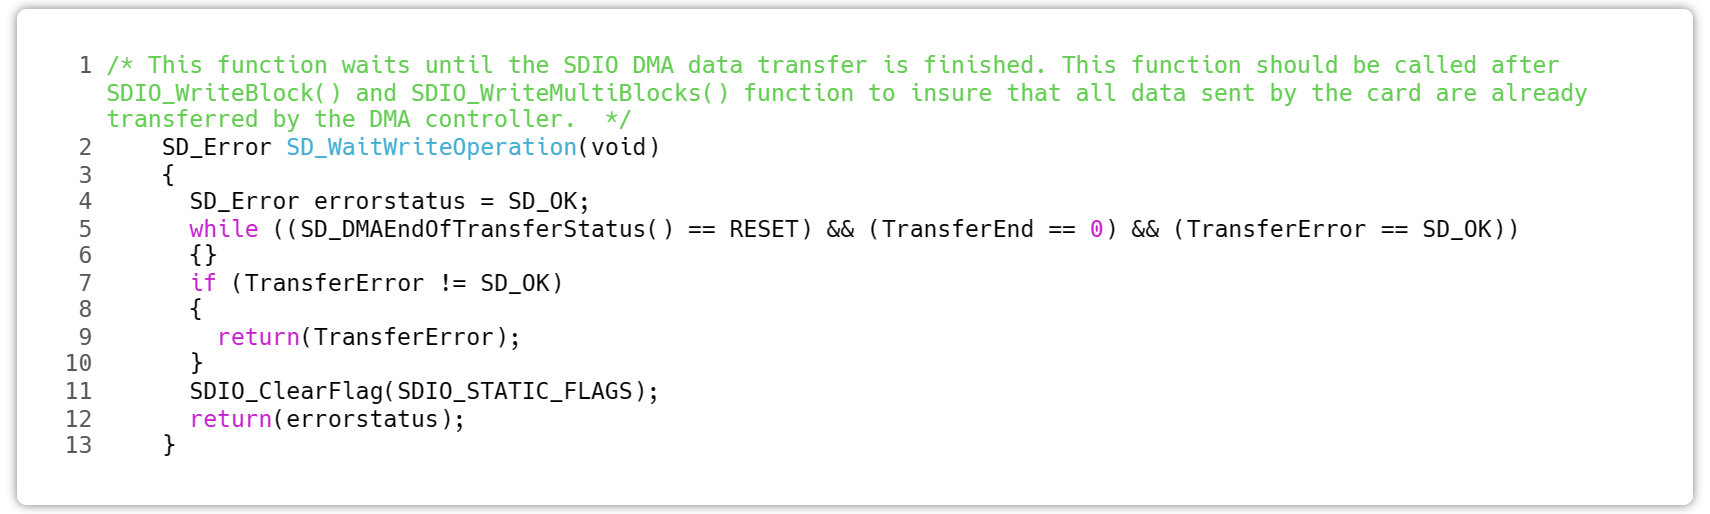
\includegraphics[width=1\textwidth]{obrazky/sample.png}
    \caption{Ukážka príkladu z~dátovej sady.}
    \label{fig:sample}
\end{figure}

\section{Analýza dátovej sady}\label{sec:dataset-analysis}
Analýza dát bola vykonaná s~cieľom získať lepšie porozumenie pre štruktúru a charakteristiku dátovej sady. Analýza zahŕňala výpočet štatistík, ako sú priemerná dĺžka distribúcia tokenov v~tele a popise funkcie a výskyt kľúčových slov jazyka v~kóde.

\begin{figure}[!ht]
    \centering
    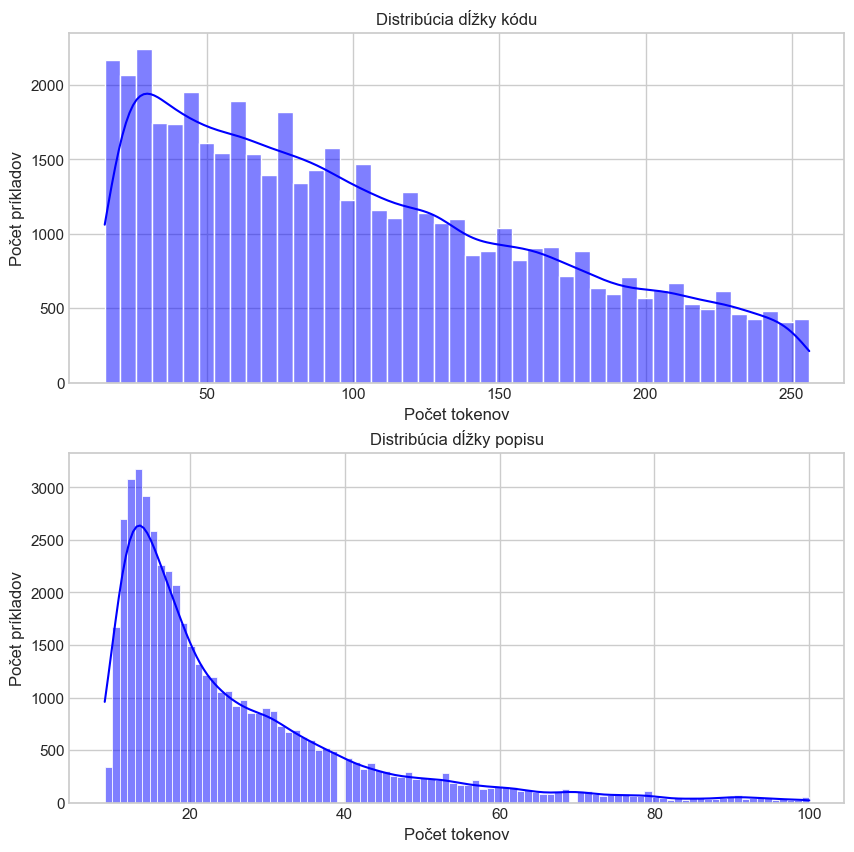
\includegraphics[width=0.7\textwidth]{obrazky/token_dist.png}
    \caption{Distribúcia počtu tokenov v~popise a tele funkcie.}
    \label{fig:token-dist}
\end{figure}

Dátová sada obsahuje celkom 6,5 milióna tokenov, z~ktorých 5,23 milióna tokenov je v~tele funkcie a 1,3 milióna tokenov je v~popise funkcie. Priemerná dĺžka popisu funkcie je 25 tokenov a priemerná dĺžka tela funkcie je 104 tokenov. Distribúcia dĺžky popisu a tela funkcie v~počte tokenov je zobrazená na obrázku~\ref{fig:token-dist}. Z~grafu je možno určiť, že väčšina popisov funkcií má dĺžku do 20 tokenov, zatiaľ čo telá funkcií majú menšiu variabilitu a väčšina z~nich má dĺžku v~rozmedzí 50 až 150 tokenov.

\begin{figure}[!ht]
    \centering
    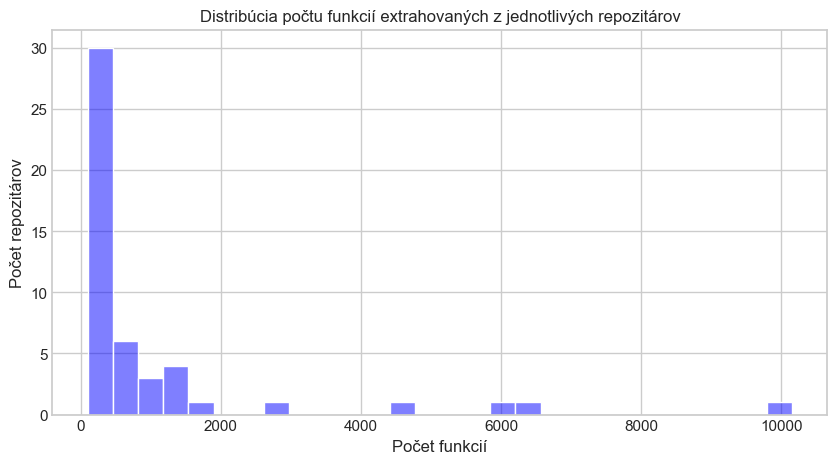
\includegraphics[width=0.7\textwidth]{obrazky/repo_dist.png}
    \caption{Distribúcia počtu funkcií extrahovaných z~jednotlivých repozitárov.}
    \label{fig:repo-dist}
\end{figure}

Na obrázku~\ref{fig:repo-dist} je zobrazený počet vzoriek z~jednotlivých repozitárov v~dátovej sade. Z~grafu je vidieť, že väčšina vzoriek pochádza z~repozitárov, ktoré majú zastúpenie v~rozmedzí do 1000 vzoriek. Najväčšie zastúpenie vzoriek v~sade má repozitár \texttt{robutest/uclinux} s~počtom viac ako 10\,000 príkladov.

\begin{figure}[!ht]
    \centering
    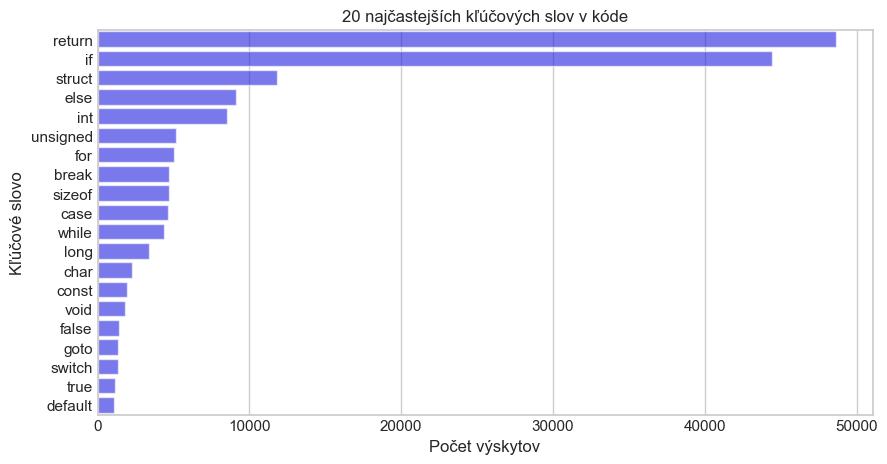
\includegraphics[width=0.7\textwidth]{obrazky/keyword_dist.png}
    \caption{Distribúcia kľúčových slov v~kóde funkcie}
    \label{fig:keyword-dist}
\end{figure}

Extrakcia kľúčových slov z~fragmentov zdrojového kódu umožňuje identifikovať opakujúce sa vzorce a posúdiť zložitosť programovania. Analýza štatistík kľúčových slov z~dátovej sady poskytuje hlbší pohľad na zdrojový kód, ktorý často závisí od riadenia toku, je presný pri manipulácii s~dátami a je systematicky štrukturovaný pri riadení systémových stavov a pamäťových operácií.

\subsection{Možné rozšírenia dátovej sady}

Pri extrakcii funkcií som zvažoval, ako pridať k~jednotlivým príkladom aj informácie o~linkovaní knižníc a ich funkcií, ktoré sú využívané v~kóde. Tieto informácie by mohli byť následne využité pri generovaní kódu, pretože by poskytli informácie o~tom, aké knižnice sú potrebné pre správne fungovanie vygenerovaného kódu. V~zozbieraných repozitároch sa nachádzalo veľké množstvo hlavičkových súborov.

Prekážkou bolo, že išlo iba o~hlavičkové súbory, ktoré obsahovali informácie o~linkovaní ďalších knižníc a vzťahy medzi jednotlivými súbormi v~projektoch boli komplikované. Rozhodol som sa túto informáciu neextrahovať, z~dôvodu nutnosti zaviesť zložitejší mechanizmus na identifikáciu a spracovanie hlavičkových súborov. Verím, že táto informácia by mohla byť doplnená v~budúcnosti, a vylepšiť tak kvalitu generovaného kódu.

Ďalším rozšírením by bola integrácia prvkov zo štandardov \textup{MISRA-C}, \textup{CERT} a podobných. Tieto smernice majú za cieľ uľahčiť vývoj bezpečného a spoľahlivého softvéru,  a predchádzať tak možným chybám v~kriticky dôležitých systémoch. Spĺňanie týchto štandardov je kľúčové v~oblasti vstavaných systémov, kde bezpečnosť a spoľahlivosť majú najvyšší význam.

Integrácia týchto smerníc by umožnila zlepšiť kvalitu dátovej sady a zabezpečila by, že vygenerovaný kód bude spĺňať prísne požiadavky na bezpečnosť a spoľahlivosť. Konkrétne by sa mohli zahrnúť pravidlá MISRA-C do procesu filtrácie vzoriek, aby sa zaistilo, že sú konformné s~týmito smernicami.

\section{Ladenie modelov}\label{sec:finetuning}

Pre ladenie, evaluáciu a inú prácu s~modelmi som vytvoril niekoľko skriptov v~jazyku Python, v~ktorých využívam rôzne knižnice, ktoré mi uľahčili prácu s~modelmi v~Jupyter zápisníkoch alebo priamo v~Python skriptoch. Platforma Hugging Face poskytuje rôzne nástroje pre prácu s~modelmi, ako sú napríklad knižnice \texttt{transformers}, \texttt{datasets} a \texttt{tokenizers}. Knižnice \texttt{transformers} a \texttt{tokenizers} poskytujú jednoduché rozhranie pre načítanie a použitie predtrénovaných modelov a tokenizérov, ktorých váhy a konfigurácie sú uložené v~repozitári Hugging Face.

Pri samotnom trénovaní som využil knižnicu \texttt{trl} (Transformer Reinforcement Learning), ktorá poskytuje jednoduché API rozhranie \texttt{SFTTrainer}. Supervised Fine-tuning Trainer, tak ako názov napovedá, je nástroj optimalizovaný pre ladenie technikou trénovania pod dohľadom. Táto knižnica natívne podporuje metódy PEFT. Okrem toho som do svojej práce začlenil \texttt{BitsAndBytesConfig} z~knižnice \texttt{transformers} pre kvantizáciu, ako aj \texttt{LoraConfig} pre nastavenia LoRA z~knižnice \texttt{peft}.

Váhy modelov \MCfim{}\footnote{\url{https://huggingface.co/xvadov01/microcoderfim-1B}\label{f1}} a \MC{}\footnote{\url{https://huggingface.co/xvadov01/microcoder-7B-q4}\label{f3}} sú voľne prístupné na verejnom úložisku.

\begin{table}[!ht]
        \footnotesize
        \centering
        \begin{tabular}{l c c}
            \hline
            \multirow{2}{*}{\textbf{Parameter}} & \multicolumn{2}{c}{\textbf{Hodnota}} \\
            & \textbf{\MC} & \textbf{\MCfim}\\
            \hline
            počet epoch & 3 & 5 \\
            \hline
            miera učenia & \makecell{$1 \times 10^{-4}$} & \makecell{$3 \times 10^{-5}$}\\
            \hline
            lr\_scheduler\_type & \makecell{constant} & \makecell{cosine}\\
            \hline
            per\_device\_batch\_size & 2 & 8\\
            \hline
            gradient\_accumulation\_steps & 1 & 8 \\
            \hline
            warmup\_ratio & 5\% & 5\%\\
            \hline
            optimalizátor & \makecell{paged 32bit \\ AdamW} & \makecell{paged 32bit \\ AdamW}\\
            \hline
        \end{tabular}
        \caption{Prehľad nastavených parametrov počas ladenia modelov.}
        \label{tab:training_settings}
    \end{table}
    
\subsection{MicroCoder}

Proces optimalizácie modelu \MC{} prebiehal pomocou ladenia, kde základný model \CL{}, ktorý som opísal v~sekcií~\ref{sec:codellama}, podstúpil ďalšiu fázu trénovania. Tento postup viedol k~vylepšeniu výkonnosti v~oblasti programovania vstavaných systémov.

V~tabuľke \ref{tab:model_size} je prehľad veľkosti modelu pred a po kvantizácii a aplikácii LoRA. Je zjavné, že kvantizácia a aplikácia LoRA viedli k~významnému zmenšeniu veľkosti. Kvantizácia umožňuje redukciu rozsahu modelu, avšak nedovoľuje trénovanie kvantizovaných váh. Pri trénovaní kvantizovaných modelov sa preto upravujú iba váhy LoRA. Tieto váhy je následne možné spojiť s~kvantizovanými, alebo pôvodnými váhami. Tento postup umožňuje načítať zmenšený model, optimalizovať vybrané projekcie a následne spojiť váhy LoRA s~váhami modelu tak, aby bolo možné využiť vzniknutý model. Takýto prístup reprezentuje efektívnu metódu ladenia, čo je zásadné v~prípade práce s~obmedzenými výpočtovými prostriedkami. Voľba QLoRA bola motivovaná analýzou vplyvu kvantizácie na výkon veľkého modelu, ktorý disponuje takmer siedmimi miliardami parametrov. Využitie kvantizačných techník mi umožnilo trénovať model na jednej grafickej karte \textsc{NVIDIA GeForce RTX~3090} s~24\,GB pamäťou. Parametre a ich nastavenia pre QLoRA adaptáciu sú v~tabuľke~\ref{tab:lora-setting}.

\begin{table}[!ht]
    \centering
    \begin{tabular}{r|c|c}
        &  \makecell{Počet \\ trénovateľných \\ parametrov} & \makecell{Veľkosť \\ (GiB)} \\
        \hline
        Základný model  & 6\,788\,878\,336      & 25,60 \\
        16bit           & 6\,788\,878\,336      & 12,80 \\
        8bit            & 6\,788\,878\,336      & 6,77 \\
        4bit            & 6\,788\,878\,336      & 3,75 \\
        LoRA $r=64$       & 33\,554\,432          & 0,064 \\
    \end{tabular}
    \caption{Porovnanie veľkosti modelu \MC{} pred a po kvantizácii a aplikácii LoRA.}
    \label{tab:model_size}
\end{table}

\begin{table}[h]
    \centering
    \begin{tabular}{l|c|p{5cm}}
        \textbf{Parameter}  & \textbf{Hodnota}
        \\ \hline
        r                   & 32        & LoRA rank, rozmer adaptácie
        \\ \hline
        lora\_alpha         & 32        & Škálovací faktor, zvyšuje vplyv nízkorozmerných matíc
        \\ \hline
        target\_modules     & Q, K, V~& Trénované projekcie dotazu, kľúča a hodnoty
        \\ \hline
        lora\_dropout       & 0,05      & Podiel váh LoRA nastavených na nulu
        \\ \hline
        Kvantizácia         & 4 bity    & Bitová hĺbka váh
        \\ \hline
        Kompresný typ       & nf4       & Formát pre ukladanie kvantizovaných váh
        \\ \hline
        Výpočtový typ       & bfloat16  &Formát pre vykonávanie výpočtov
    \end{tabular}
    \caption{Nastavenia metódy QLoRA pre trénovanie modelu \MC{}.}
    \label{tab:lora-setting}
\end{table}


Pri trénovaní bola použitá konštantná miera učenia $1 \times 10^{-4}$, čo umožnilo slabú, ale stabilnú konvergenciu počas celého procesu trénovania. Veľkosť dávky bola nastavená na~2, čo optimalizovalo využitie pamäte GPU a zároveň udržiavalo efektívny tok. Nakoľko GPU \textsc{GeForce RTX 3090} má obmedzenú kapacitu pamäte, akumulácia gradientov bola nastavená na 1, čo umožnilo pravidelné aktualizácie váh bez nadmerného zaťaženia pamäte.

Celkový počet epoch bol určený na 3 a proces zabral 15\,h a 28\,m. Zahrievací pomer bol nastavený na 5\%, čo zabezpečuje plynulé zvyšovanie miery učenia na začiatku trénovania a predchádza príliš rýchlym a nestabilným zmenám vo váhach.

V~tabuľke \ref{tab:training_settings} je uvedený prehľad nastavených hyper-parametrov ladenia modelu \MC{}.


\begin{figure}[!ht]
    \centering
    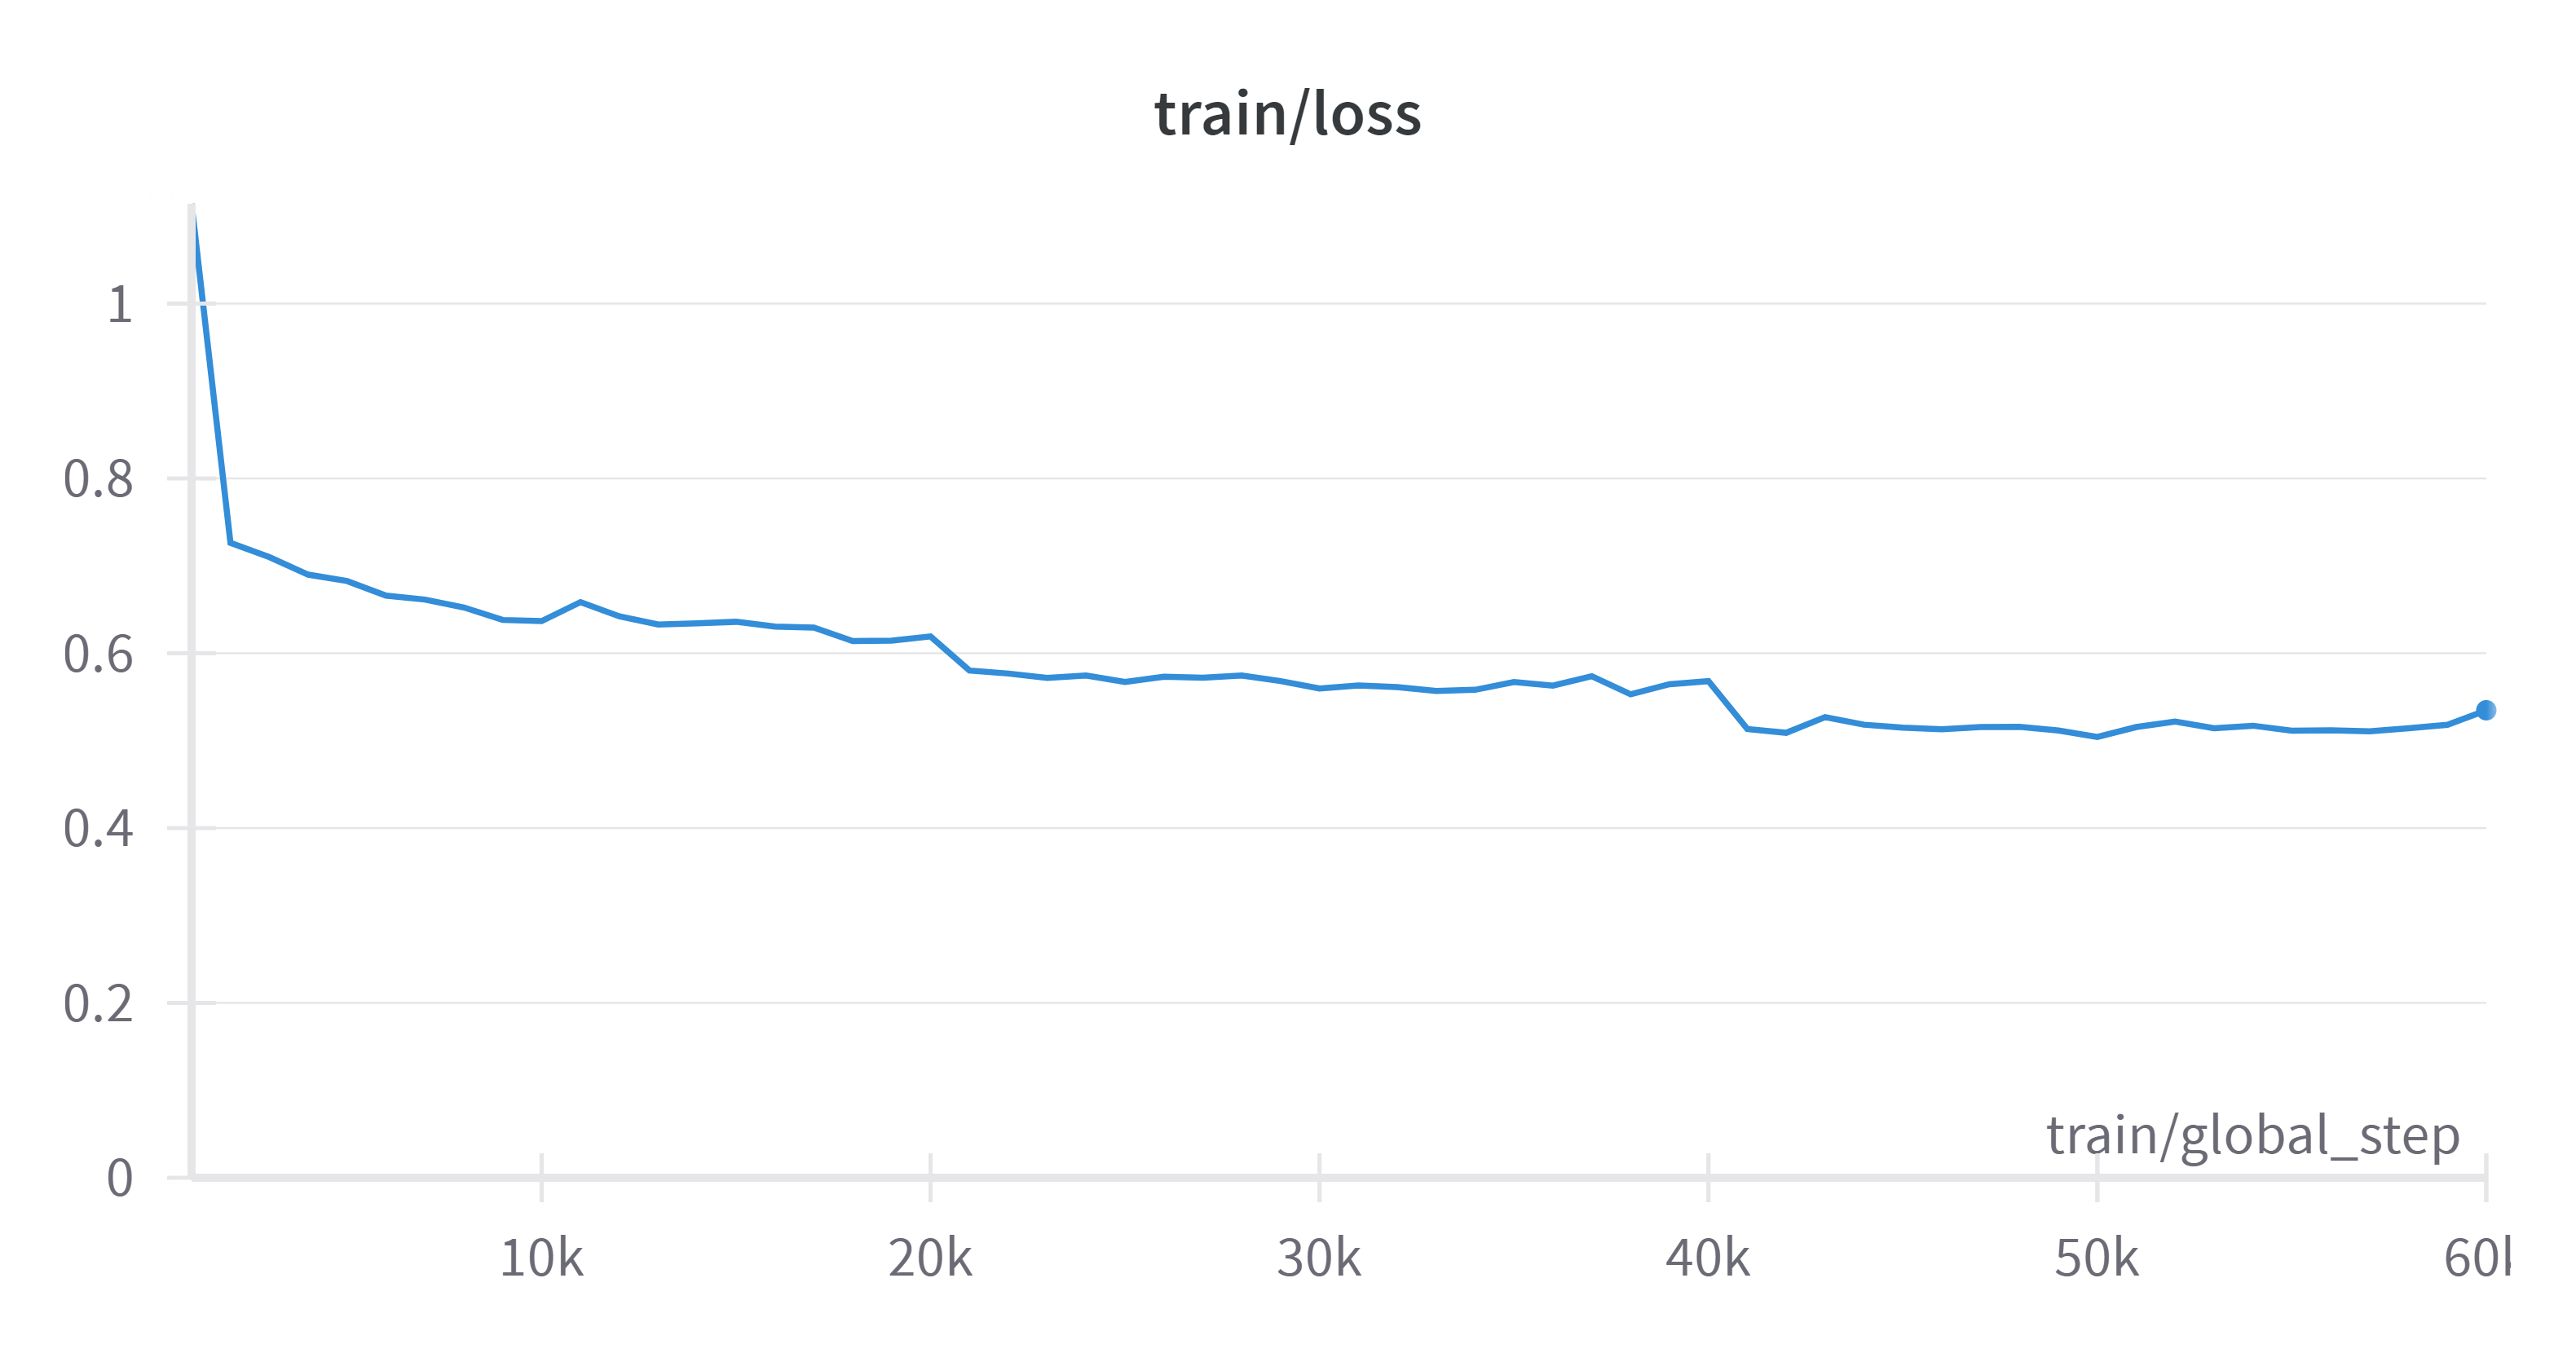
\includegraphics[width=0.45\textwidth]{obrazky/CodeLlama_TL.png}
    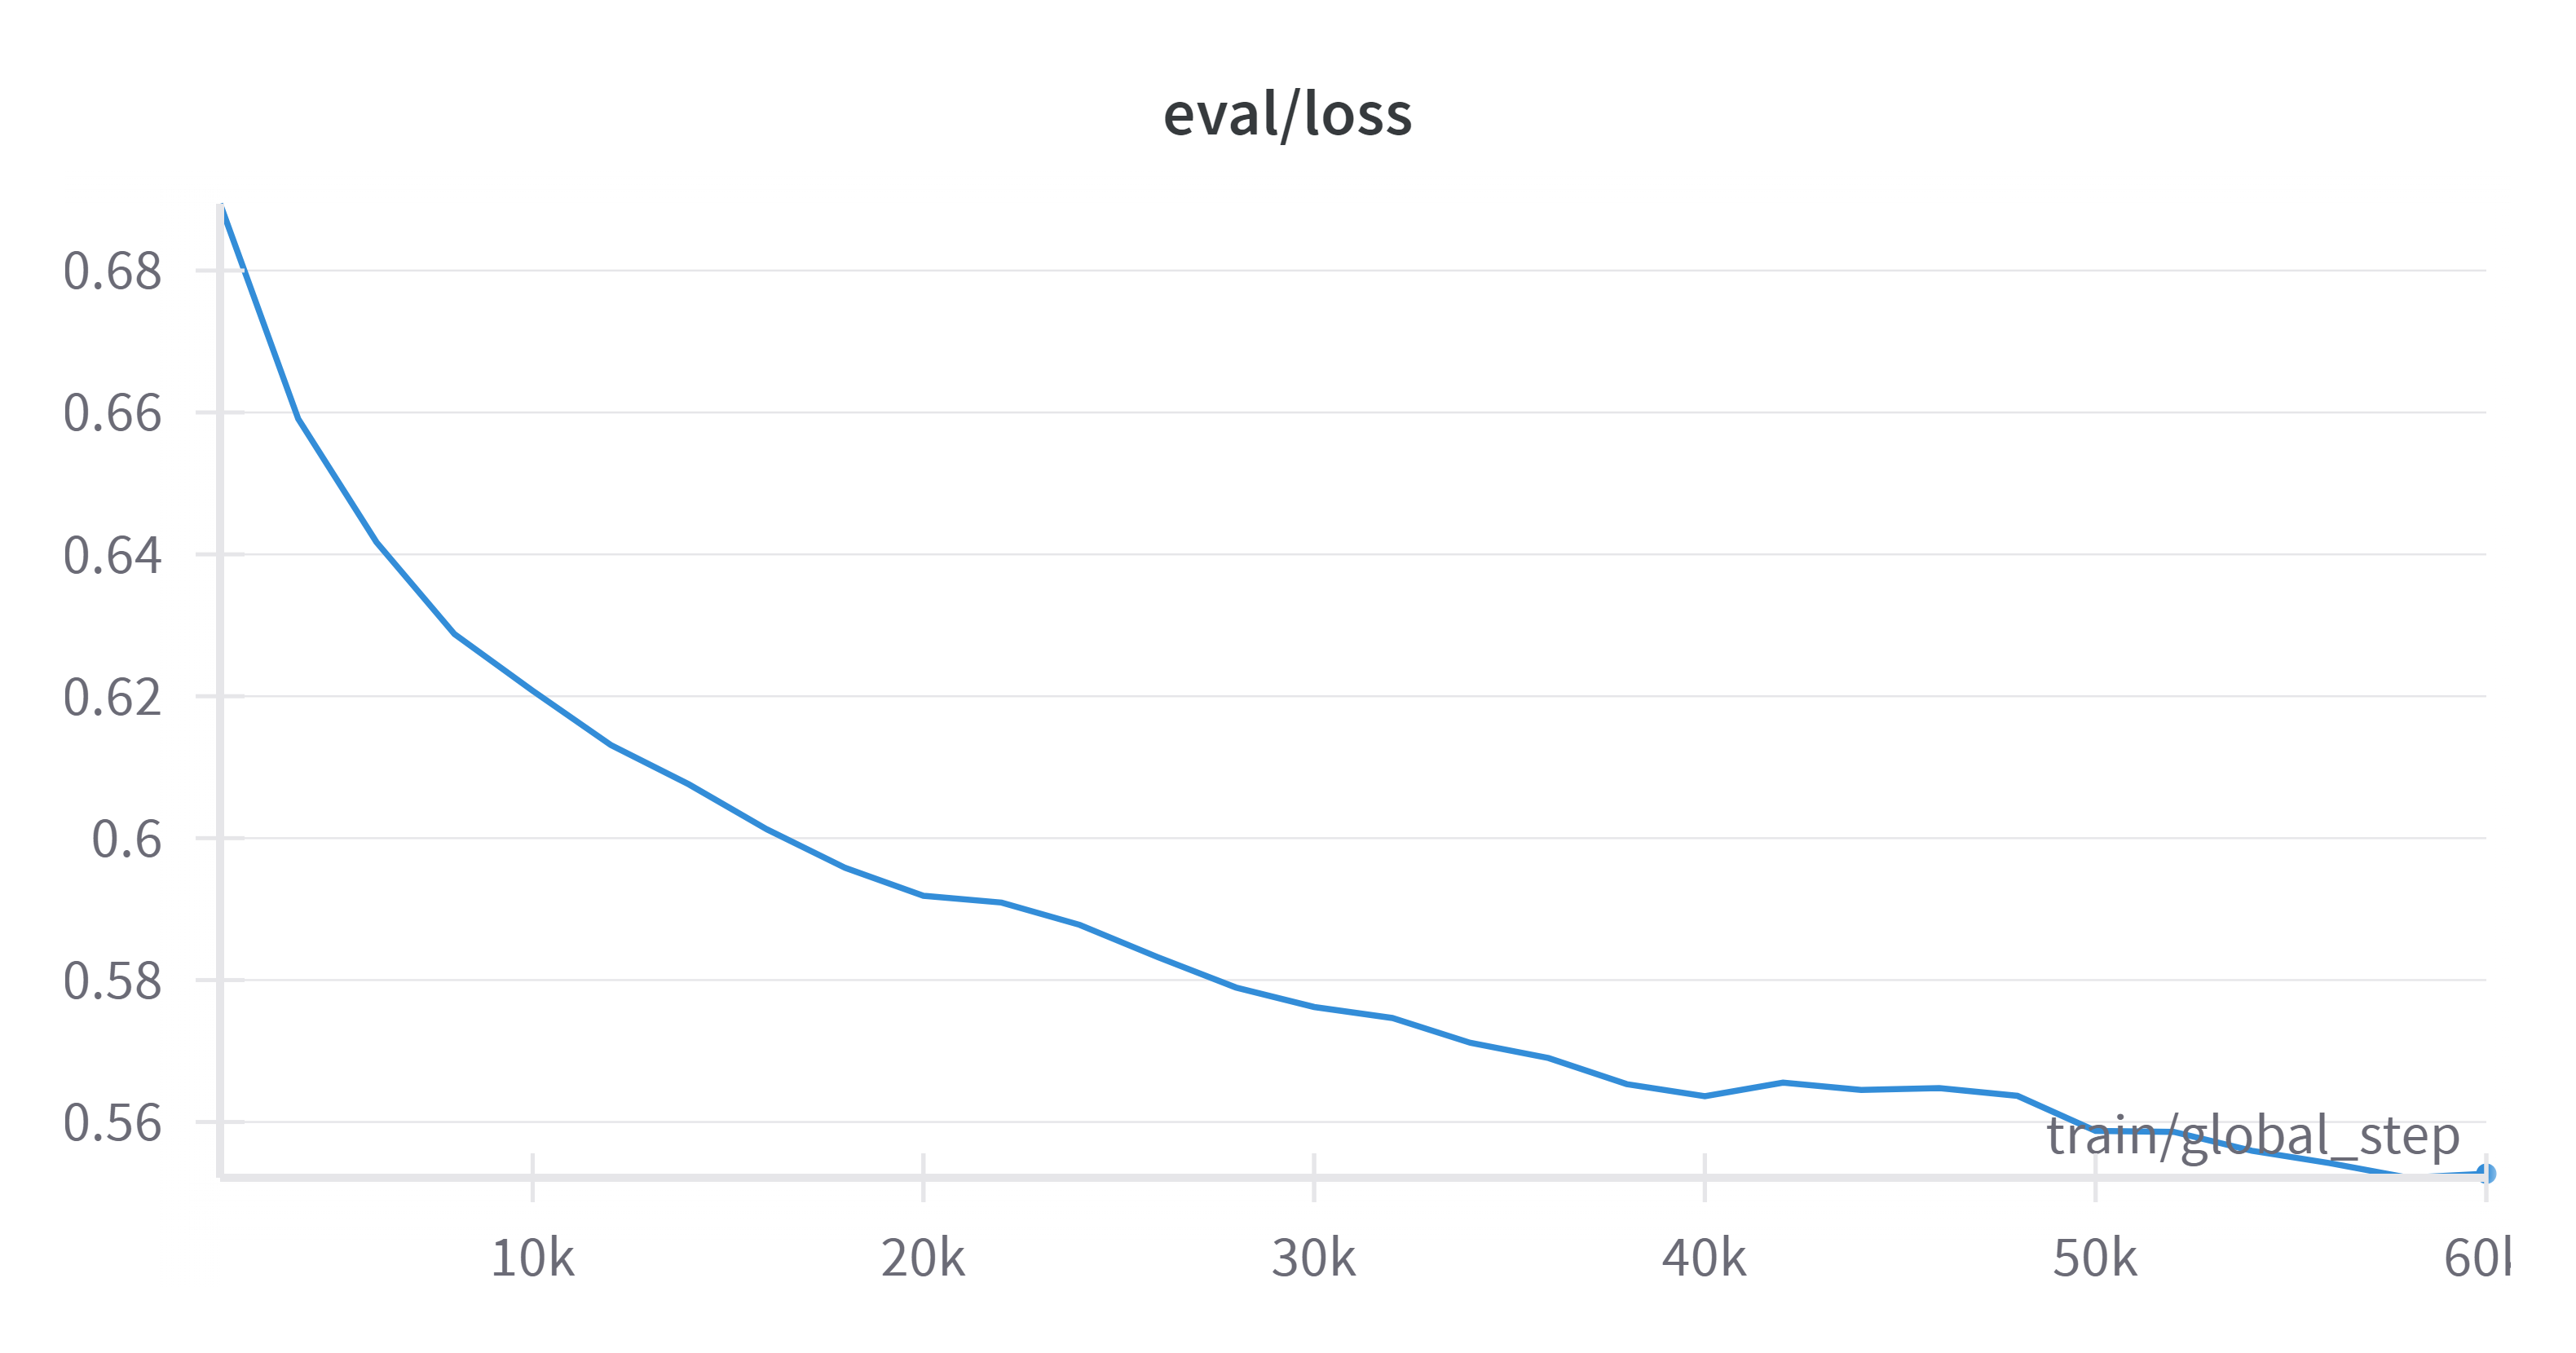
\includegraphics[width=0.45\textwidth]{obrazky/CodeLlama_EL.png}
    \caption{Graf zobrazujúci trénovaciu a validačnú stratu modelu \MC{} počas viacerých epoch, ilustrujúc pokrok v~učení a hodnotenie výkonnosti modelu.}
    \label{fig:MicroCoderFTGraphs}
\end{figure}

\subsection{MicroCoderFIM}\label{sec:microcoderfim-training}

Pre druhú fázu ladenia som vybral model \SC{}, podrobne opísaný v~sekcií~\ref{sec:starcoder}. Výber tohto modelu bol motivovaný jeho menšou komplexitou a relatívne jednoduchšou trénovateľnosťou. Táto vlastnosť umožnila experimentovanie s~trénovaním všetkých váh pri zachovaní 32-bitovej presnosti. Proces ladenia modelu bol realizovaný na grafickej karte \textsc{NVIDIA GeForce RTX 3090} po dobu 5 hodín a 25 minút. Pri ladení bola nastavená miera učenia $3 \times 10^{-5}$ a ďalšie parametre, ktoré sú podrobným spôsobom uvedené v~tabuľke~\ref{tab:training_settings}.

\subsubsection*{Príprava vzoriek do formátu pre trénovanie}

Na trénovanie modelu som použil rovnakú dátovú sadu ako pri trénovaní modelu \MC, ale s~iným prístupom k~príprave vzoriek. Model bol trénovaný na úlohe FIM a bolo potrebné pripraviť vzorky do formátu SPM (Suffix-Prefix-Middle) alebo PSM (Prefix-Suffix-Middle). Pre tieto účely som adaptoval funkciu \verb|permute|, ktorú som prebral z~\cite{Allal2023}. Vstup do funkcie je kód spolu s~textovým popisom funkcie. Výsledok je text obohatený o~tokeny, ktoré označujú oddelenie jednotlivých častí. Používam pravdepodobnosť transformácie FIM 100\%, čo znamená, že všetky vzorky sú transformované do formátu FIM. Dĺžka jednotlivých častí je $\frac{1}{3}$ s~náhodným posunom o~maximálne 10\% dĺžky vzorky. Pre inferenciu som využil len časť po token <MID> tak, aby model dostal informáciu, že má nasledovať stredná časť, ktorú následne generuje.

\noindent Tokenizovaný vstup pre trénovanie potom nadobúda jeden z~formátov:
\begin{center}
    \textbf{<PRE>(prefix)<SUF>(suffix)<MID>(middle)}\\
    \textbf{<PRE><SUF>(suffix)<MID>(prefix)(middle)}
\end{center}

\begin{figure}[!ht]
    \centering
    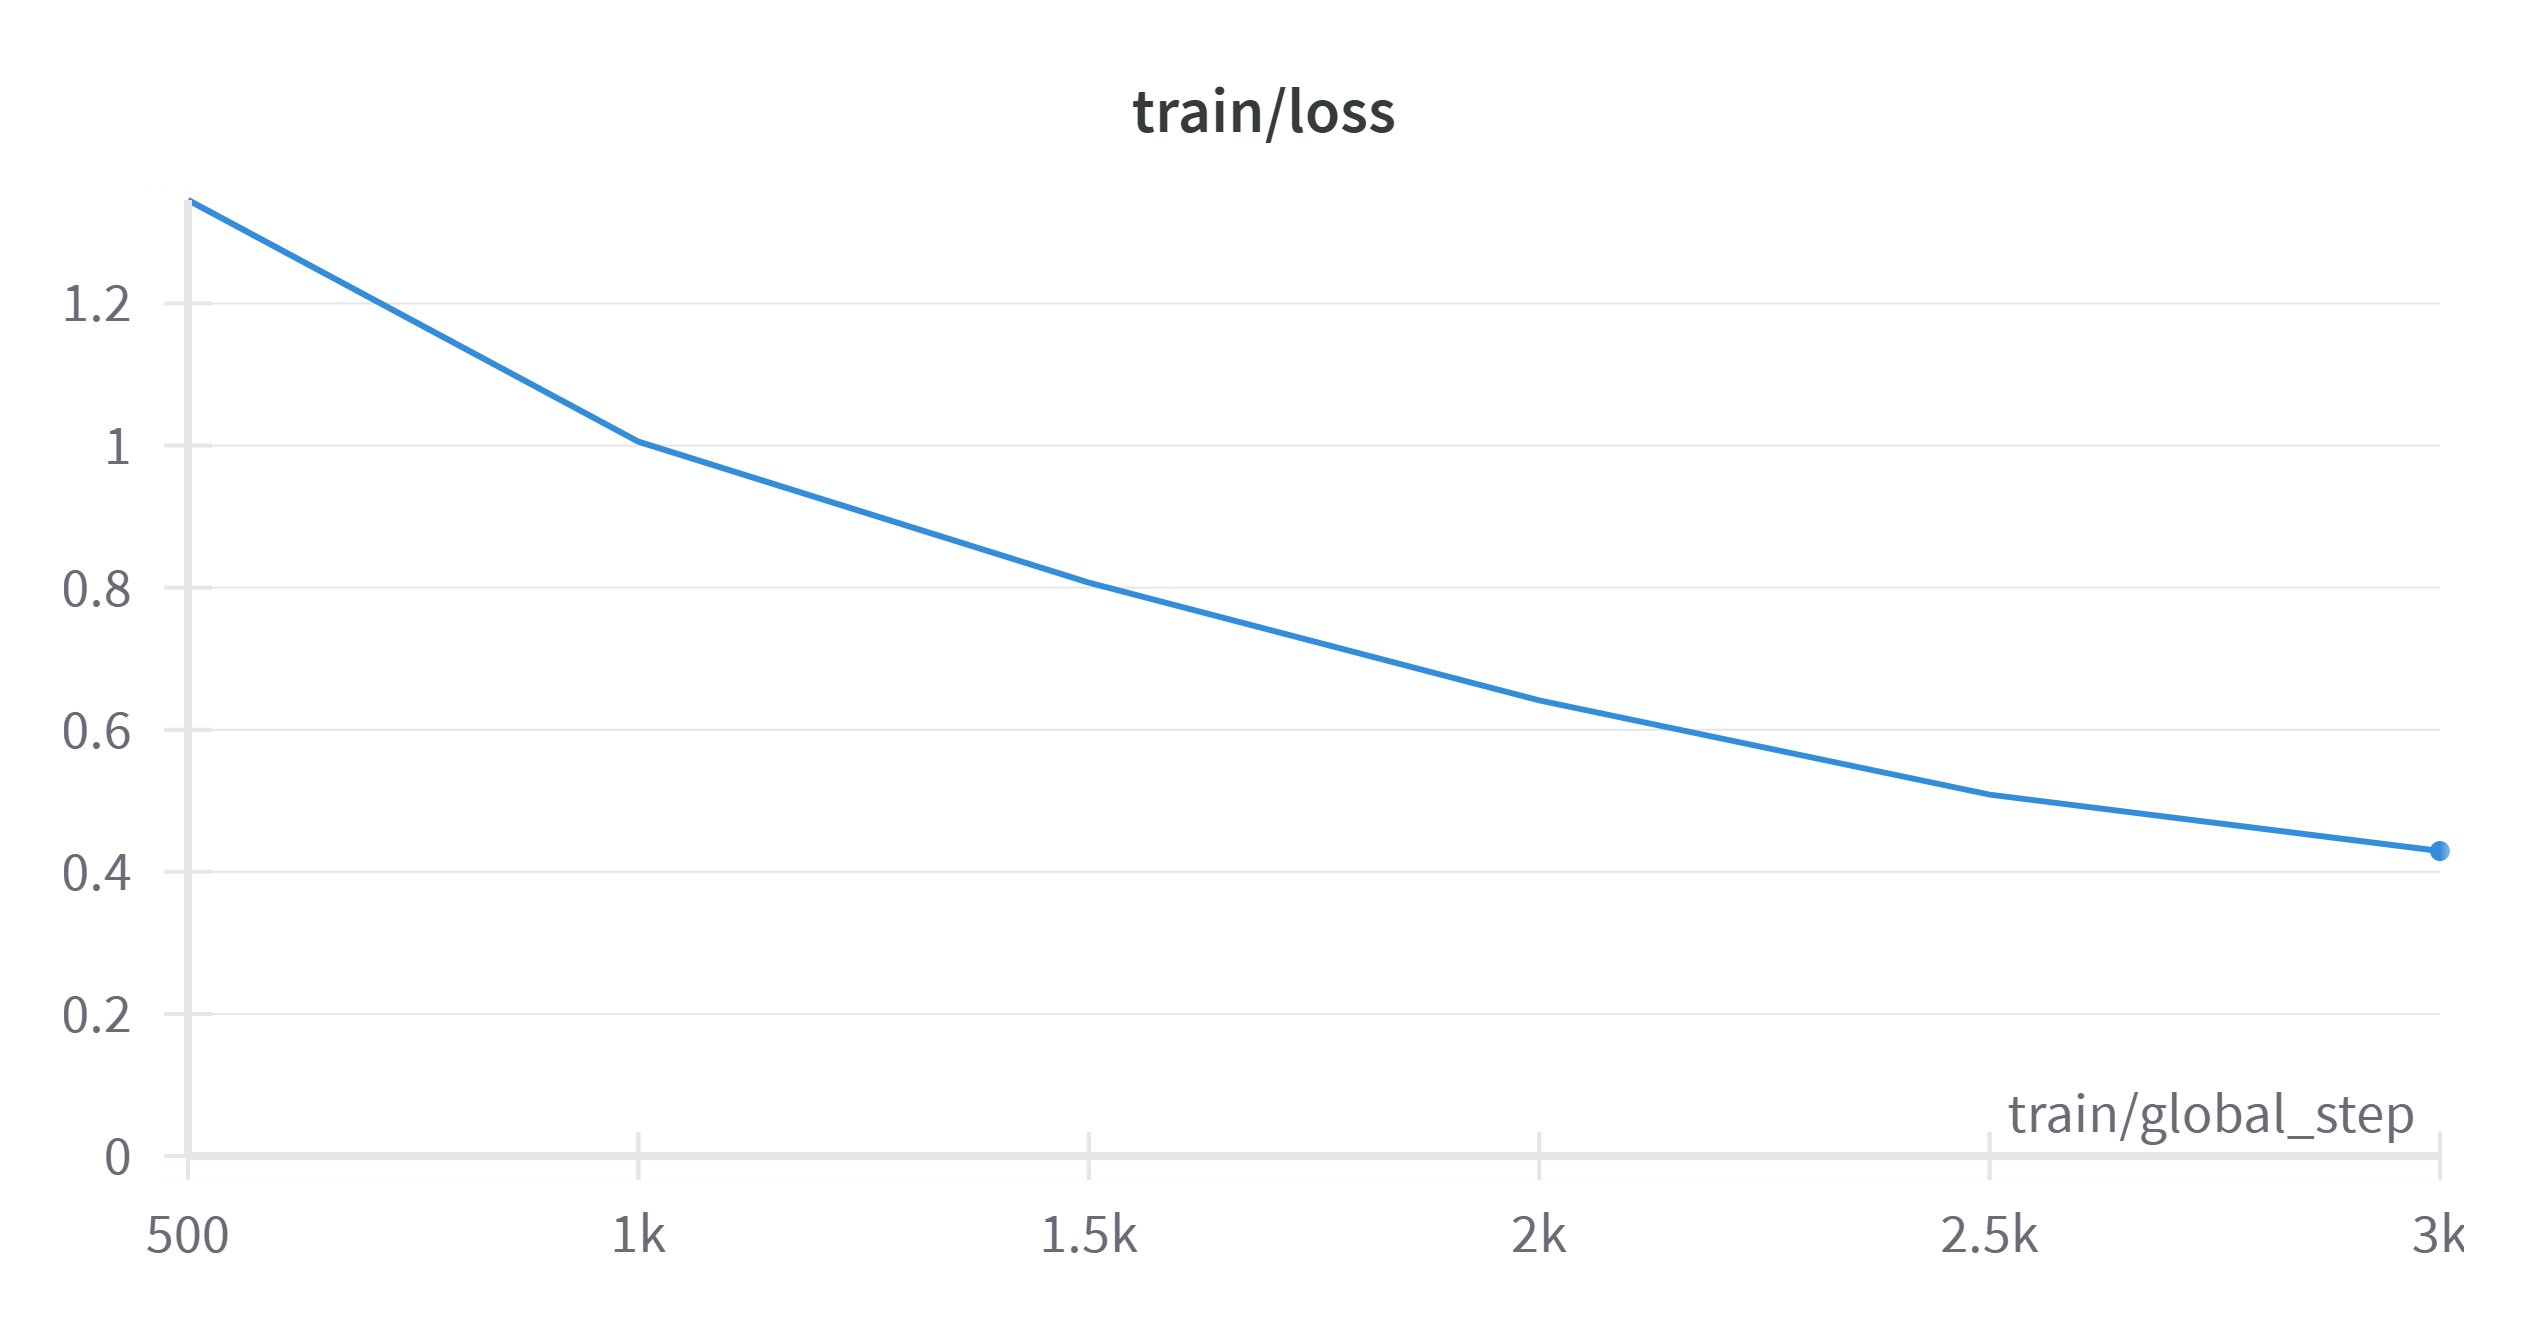
\includegraphics[width=0.45\textwidth]{obrazky/MicroCoderFIM-TL.png}
    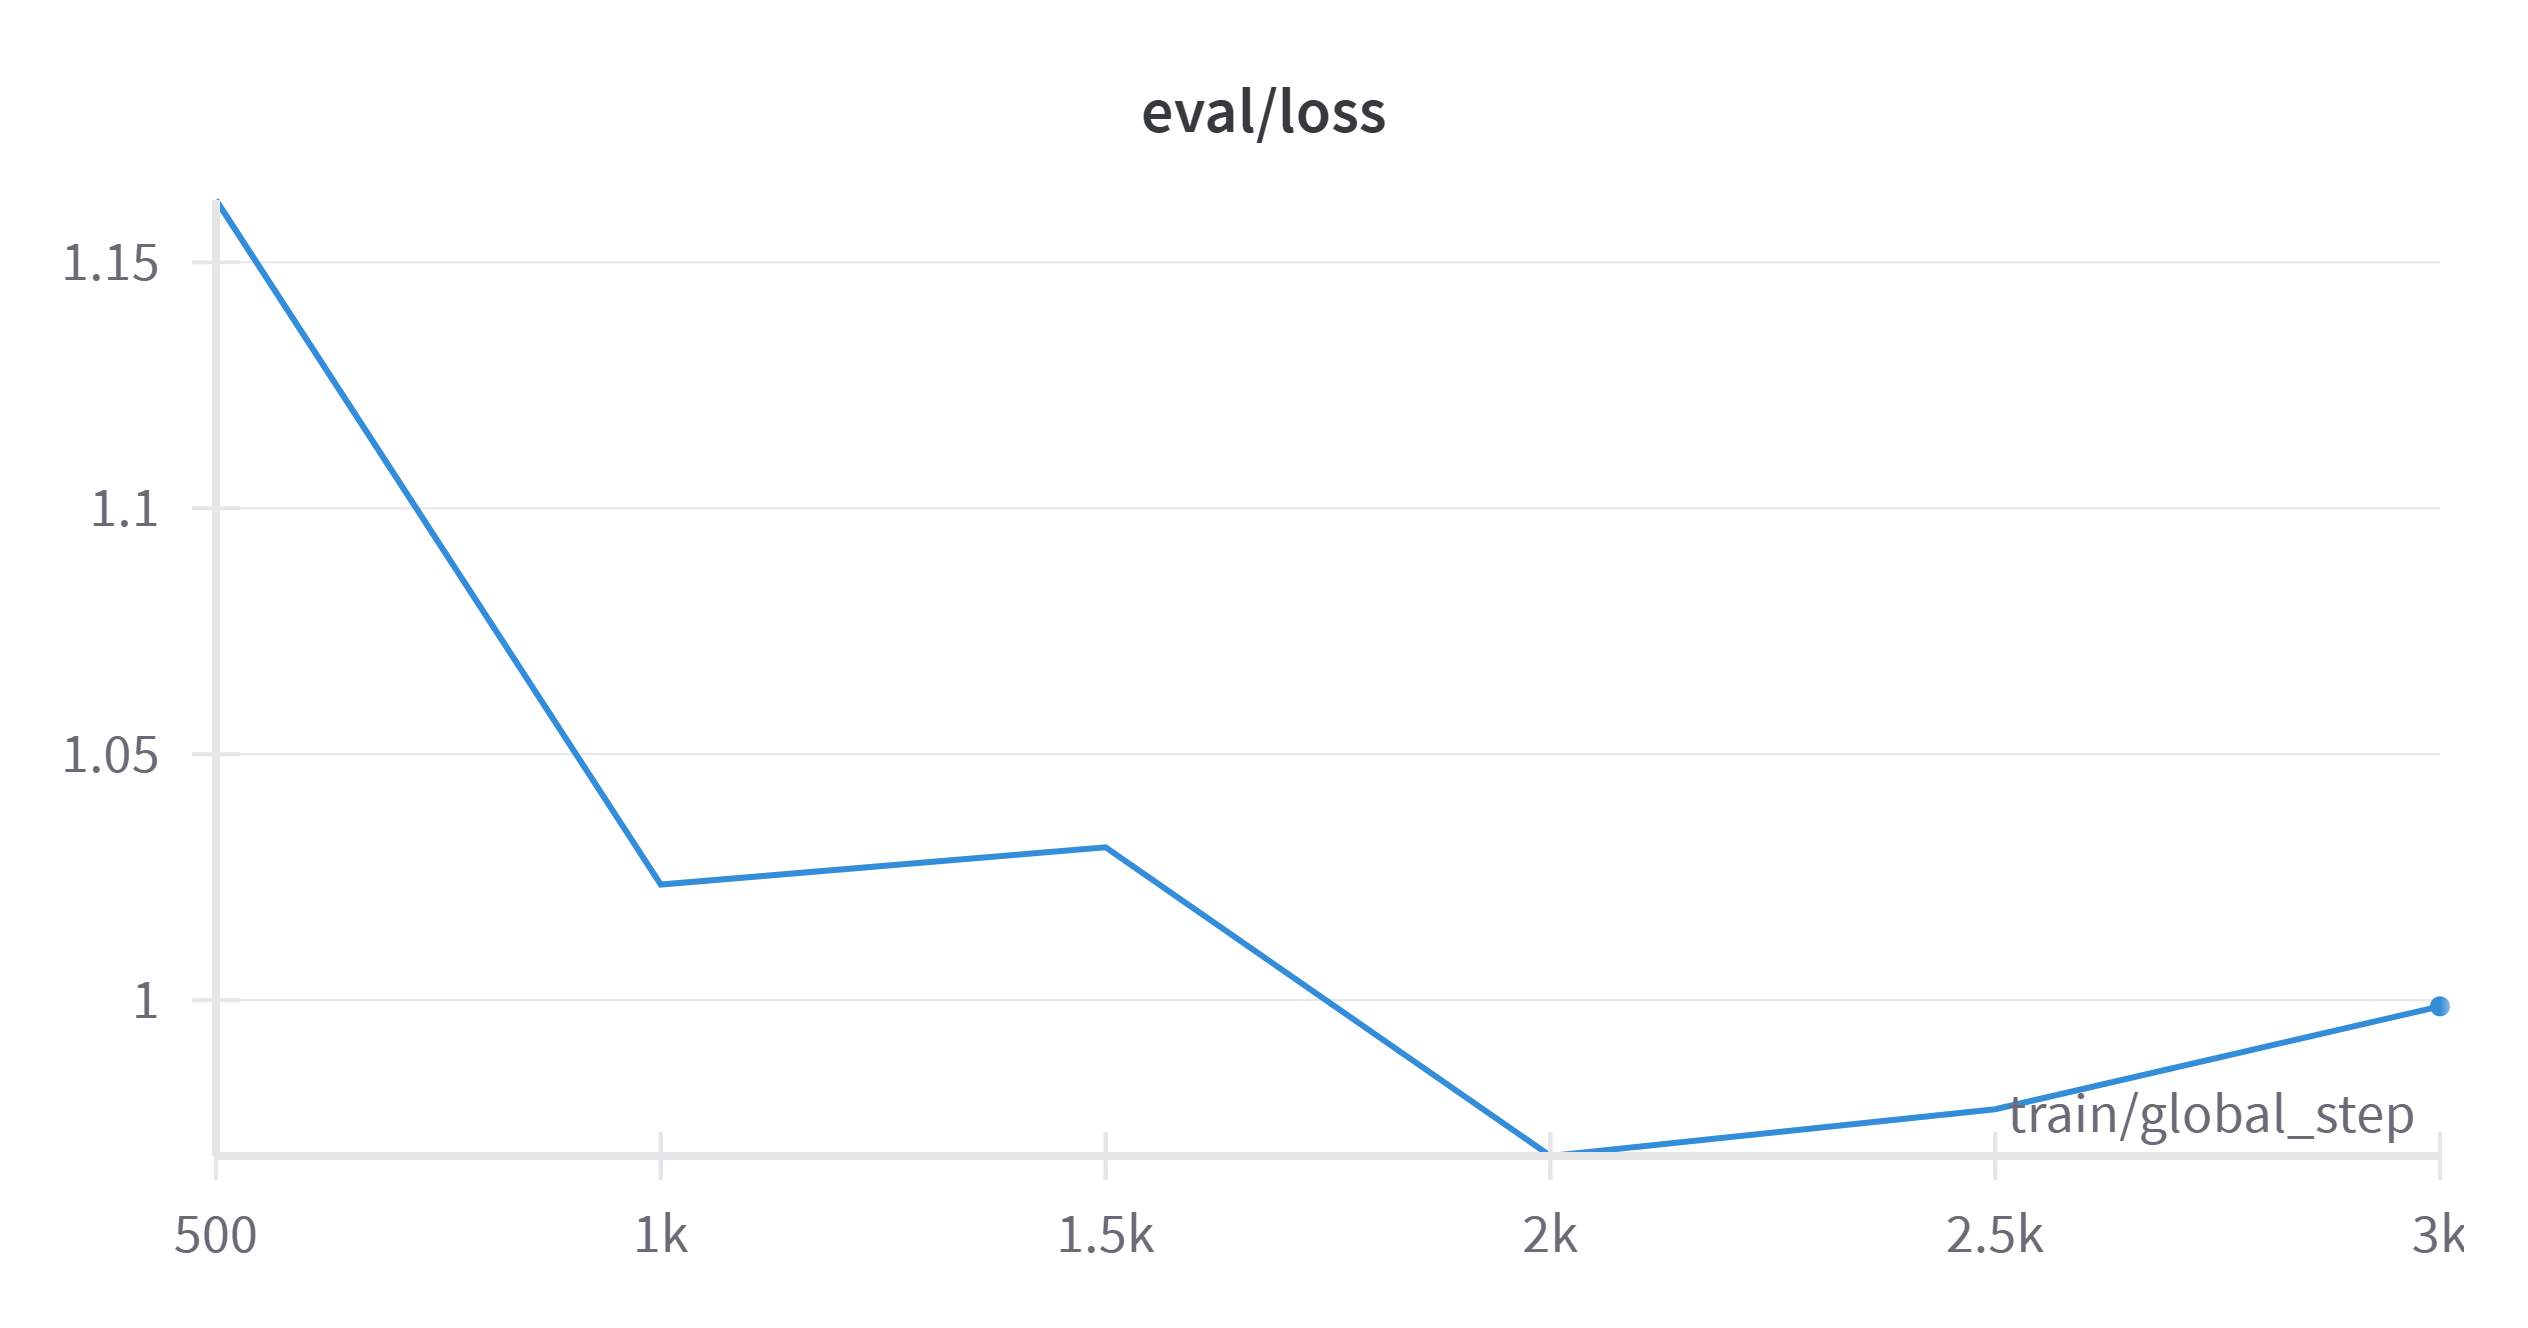
\includegraphics[width=0.45\textwidth]{obrazky/MicorCoderFIM-EL.png}
    \caption{Graf trénovacej a validačnej straty modelu \MCfim{}. Trénovacia strata postupne klesá, zatiaľ čo validačná strata spočiatku jemne klesá, ale následne stúpa. Tento jav naznačuje možný výskyt preučenia. Model dobre funguje na trénovacích dátach, ale jeho schopnosť generalizovať na nové, nevidené dáta, je obmedzená.}
    \label{fig:MicroCoderFIMFTGraphs}
\end{figure}

\subsection{Emisie CO2}

 Uvádzam uhlíkovú stopu~\cite{lacoste2019quantifying} modelov \MC{} a \MCfim{}, s~cieľom porovnať ich efektivitu a environmentálny dopad. Obidva modely boli trénované na grafickej karte \textsc{NVIDIA GeForce RTX 3090}, čo umožňuje priame porovnanie ich energetických nárokov a súvisiacich emisií CO\textsubscript{2}. Jednotka CO\textsubscript{2}eq (ekvivalent oxidu uhličitého) predstavuje štandardný spôsob vyjadrenia rôznych typov skleníkových. Zohľadňuje relatívny vplyv na globálne otepľovanie konvertovaním množstva plynov na ekvivalentné množstvo oxidu uhličitého s~rovnakým potenciálom globálneho otepľovania~\cite{EEAGlossary2023}.

Model \MC{} bol trénovaný po dobu 15,5 hodiny, počas ktorej vyprodukoval celkovo 2,34 kg CO\textsubscript{2}eq. Model \MCfim{} vyžadoval menej trénovacieho času, konkrétne 5,5 hodiny, a jeho celkové emisie CO\textsubscript{2}eq dosiahli 0,83 kg. Tieto údaje sú základom pre ďalšie diskusie o~efektivite a environmentálnom vplyve pri vývoji jazykových modelov. Rozdiel v~emisiách je značný a poukazuje na potenciálnu úsporu energie pri optimalizácii menších jazykových modelov.

\section{Evaluácia modelov}\label{sec:evaluation}

Ladené modely som vyhodnotil na testovacej sade, ktorá pozostávala z~10\% vzoriek z~pôvodnej dátovej sady. Pre evaluáciu kvality modelov som využil metriky BLEU~\cite{post-2018-call}, CodeBLEU\footnote{https://github.com/k4black/codebleu}, chrF{++}~\cite{post-2018-call} a  ROUGE-L\footnote{https://github.com/google-research/google-research/tree/master/rouge}. Tieto metriky som zvolil na základe zistení práce~\cite{evtikhiev2020out}, ktorá zároveň tvrdí, že metrika chrF{++} vykazuje najvyššiu koreláciu s~ľudským hodnotením. Skóre modelu \MC{} som vypočítal zo vzorky 1000 príkladov kvôli dlhšiemu času inferencie. Pre \MCfim{} som použil všetkých 5025 príkladov z~testovacej sady. Výsledky evaluácie sú zhrnuté v~Tab.~\ref{tab:results}.

\noindent Detaily k~použitej implementácií a parametrom použitých metrík:
\begin{description}
    \item[CodeBLEU]  Nastavenie váh $\alpha =\beta = \gamma =\delta = 0.25$, špecifikovaný programovací jazyk C++.
    \item[ChrF] Parametre boli zvolené tak, aby zodpovedali metrike ChrF++ (nastavené bigramy slov a 6-gramy znakov).
\end{description}

\begin{table}[!ht]
    \footnotesize
    \centering
    \begin{tabular}{@{}c|rlcccc@{}}
        \multirow{2}{*}{\textbf{Úloha}} & \multirow{2}{*}{\textbf{Model}} & \multirow{2}{*}{} & \multicolumn{4}{c}{\textbf{Metriky}} \\
        & & & BLEU & CodeBLEU & CHRF++ & ROUGE-L \\ \hline
        \multirow{4}{*}{NL\,-\,PL} & \textsc{\textsc{GPT-3.5 Turbo}} & 175B & \textbf{15,21} & 15,00 & \textbf{25,92} & \textbf{27,84} \\
        & \CL{} & 7B & 4,67 & \textbf{18,40} & 19,50 & 16,10 \\
        & \textsc{DeepSeek-Coder} & 6.7B & 9,63 & 17,18 & 25,79 & 18,45 \\
        & \MC{} & 7B & 10,43 & 16,85 & 25,33 & 20,84 \\
        & \MC{}\tablefootnote{Model vzniknutý zlúčením LoRA váh do 16-bitového modelu.} & 7B & 8,24 & 17,49 & 24,92 & 17,55 \\
        % & \MCfim{} & 1B & 16.50 & 15.25 & 29.52 & 21.77 \\
        \hline
        \multirow{2}{*}{FIM} & \SC{} & 1B & 11,85 & 11,58 & 19,54 & 19,18 \\
        & \MCfim{} & 1B & \textbf{31,74} & \textbf{40,53} & \textbf{51,54} & \textbf{43,31} \\
    \end{tabular}
    \caption{Tabuľka výsledkov inferencie modelov na testovacej sade.}
    \label{tab:results}
\end{table}

Pre porovnanie som vyhodnotil aj model \textsc{ChatGPT}. Pri vygenerovaní výsledkov bolo použité OpenAI API a model \textsc{GPT-3.5 Turbo}. Model dostal zadanie, aby generoval iba telo funkcie, bez dodatočných komentárov, ktoré tento model generuje kvôli technike posilňovaného učenia. Keďže ako referenčný výstup používam iba kód funkcie, bolo potrebné očistiť výstup tak, aby bola dosiahnutá najvyššia miera objektivity a až následne vypočítať skóre. Model bol vyhodnotený iba na vzorke 2000 testovacích príkladov z~testovacej sady.

\begin{figure}[H]
    \centering
    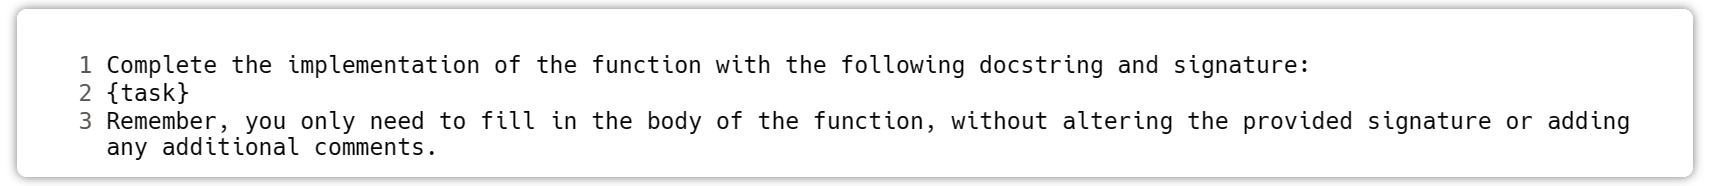
\includegraphics[width=1\textwidth]{obrazky/gpt-prompt.png}
    \caption{Formát promptu použitý pre model \textsc{GPT-3.5 Turbo}.}
    \label{fig:gpt-prompt}
\end{figure}

\subsection{MicroCoder}

Tento model si aj napriek nízkym výsledkom základného modelu polepšil iba o~niekoľko percent vo všetkých metrikách okrem CodeBLEU. Aj keď výsledky ukazujú, že výstupy modelu sa vzdialene približujú referenčným výstupom, ukážky kódu~\ref{code:MicroCoder_1} a~\ref{code:MicroCoder_2} ukazujú, že model je schopný generovať syntakticky korektný kód, ktorý do určitej miery rešpektuje popis funkcie.

Adaptácia modelu na novú úlohu je v~porovnaní s~modelom \MCfim{} podstatne slabšia, ako ukazuje tabuľka~\ref{tab:results}. Tento fakt môže byť spôsobený tým, že model bol trénovaný po menší počet epoch. Ďalším možným faktorom je použitie kvantizácie a nízkorozmerných matíc LoRA, ktoré mohli znížiť schopnosť modelu efektívne sa prispôsobiť novej úlohe v~porovnaní s~modelom \MCfim{}, ktorý prešiel trénovaním všetkých váh bez kvantizácie.

Bežný postup je ladenie LoRA matíc s~využitím kvantizovaných váh modelu a následné spojenie 16-bitového adaptéru s~modelom, ktorý je v~32 alebo 16-bitovej hĺbke. Pri testovaní modelov po zlúčení vykazovalo spojenie adaptéru so 16-bitovými váhami modelu v~priemere o~2\% horšie výsledky, ako zlúčenie s~kvantizovanými váhami. Rozhodol som sa preto zlúčiť LoRA adaptér s~kvantizovaným modelom, čím vznikol \MC{}.

Všimol som si, že pri práci s~kvantizovaným modelom sú rozdiely medzi rôznymi inicializáciami váh modelu výraznejšie a model sa môže ľahšie uväzniť v~lokálnom optimálnom bode. Pri inicializácii váh následného modelu totiž dochádza k~zníženiu presnosti reprezentácie váh. Malé zmeny vo váhach môžu spustiť reťazovú reakciu, ktorá vedie k~zhoršeniu výsledkov. V~prílohe~\ref{app:more-results} sú detailnejšie popísané niektoré výstupy a problémy kvantizovaného modelu.

\begin{figure}
    \centering
    \raisebox{-\height}{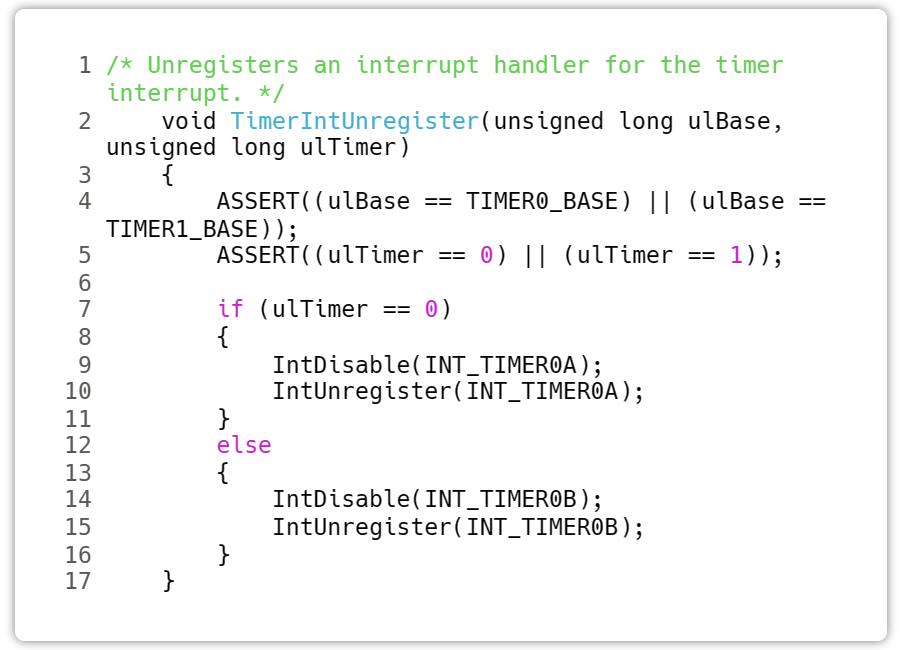
\includegraphics[width=0.45\textwidth]{obrazky/mc76.png}}
    \raisebox{-\height}{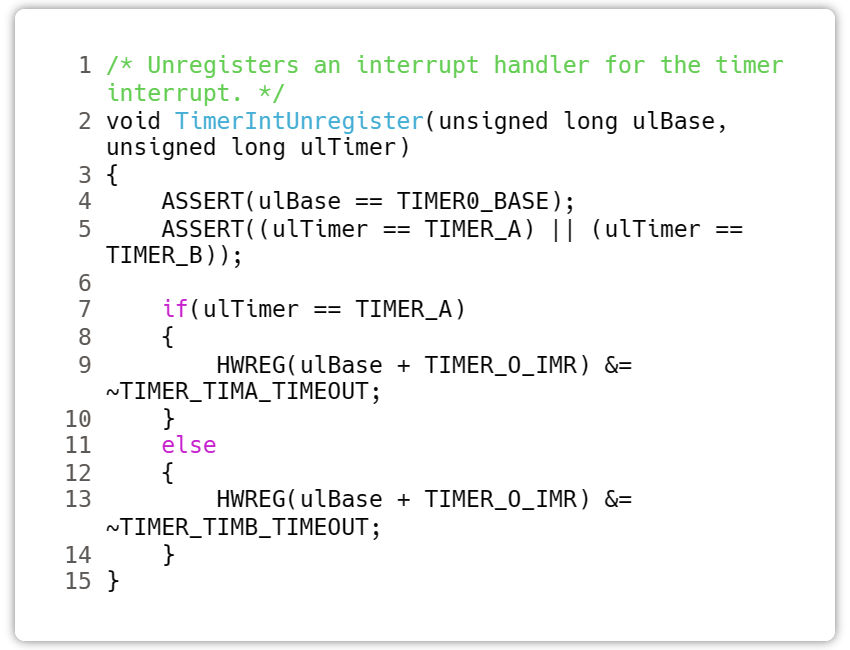
\includegraphics[width=0.45\textwidth]{obrazky/gpt76.png}}
    \caption{Výstup modelu \MC{} (vľavo) a výstup nástroja Github Copilot očistený o~sprievodné komentáre (vpravo) pre rovnaký príklad.}
    \label{code:MicroCoder_1}
\end{figure}

\begin{figure}[H]
    \centering
    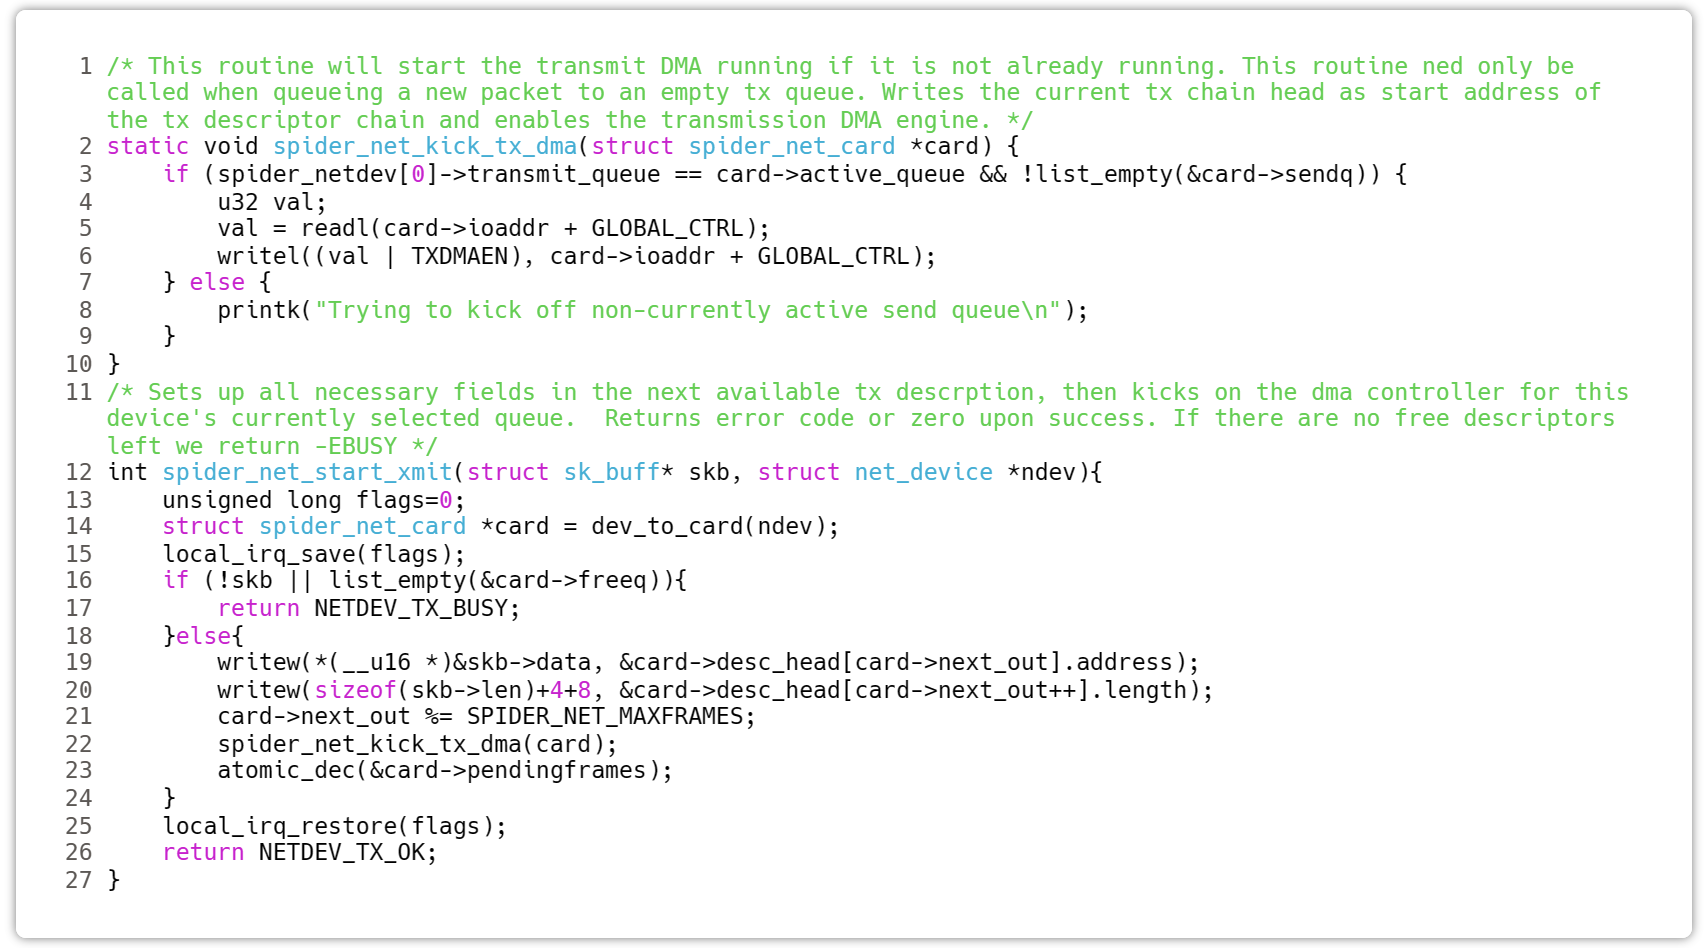
\includegraphics[width=0.9\textwidth]{obrazky/mc69.png}
    \caption{Výstup modelu \MC.}
    \label{code:MicroCoder_2}
\end{figure}

Výstup modelu na obrázku~\ref{code:MicroCoder_2} ilustruje jeho schopnosť manipulovať s~generickými hardvérovými funkciami, ako sú \texttt{local\_irq\_save} a \texttt{writel}. Zároveň je pozoruhodný plynulý prechod medzi funkciami, ktoré model vygeneroval a prepojil dva logické celky kódu.

\subsection{MicroCoderFIM}

Výsledky modelu \MCfim{} ukazujú výrazné zlepšenie vo všetkých metrikách v~porovnaní so základným modelom. Tento model dosiahol najlepšie výsledky vo všetkých metrikách, čo naznačuje, že sa dokázal efektívne adaptovať na novú úlohu. Ukážky kódu~\ref{code:MicroCoderFIM_1} naznačujú schopnosť efektívne dopĺňať kód v~kontexte a zachovávať jeho funkcionalitu.

Proces trénovania trval dlhšie ako pri skôr spomínanom modeli. Platí, že miera učenia bola nižšia a nebola konštantná, ale bola nastavená na kosínusovú mieru učenia, čo znamená, že dochádzalo k~jej postupnému znižovania počas trénovania.

V~rámci experimentálnej časti práce som vykonal rozsiahle testovanie modelu, aby som identifikoval optimálne parametre pre generovanie textu. Podrobnosti experimentov a ich výsledky sú detailne popísané v~prílohe~\ref{app:fim_test}, ktorá obsahuje analýzu vplyvu rôznych nastavení parametrov, ako sú teplota (temperature), maximálna dĺžka generovanej sekvencie (max\_new\_tokens) a pravdepodobnosť výberu (top\_p), na výkonnosť modelu pri generovaní textu.

\begin{figure}[H]
    \centering
    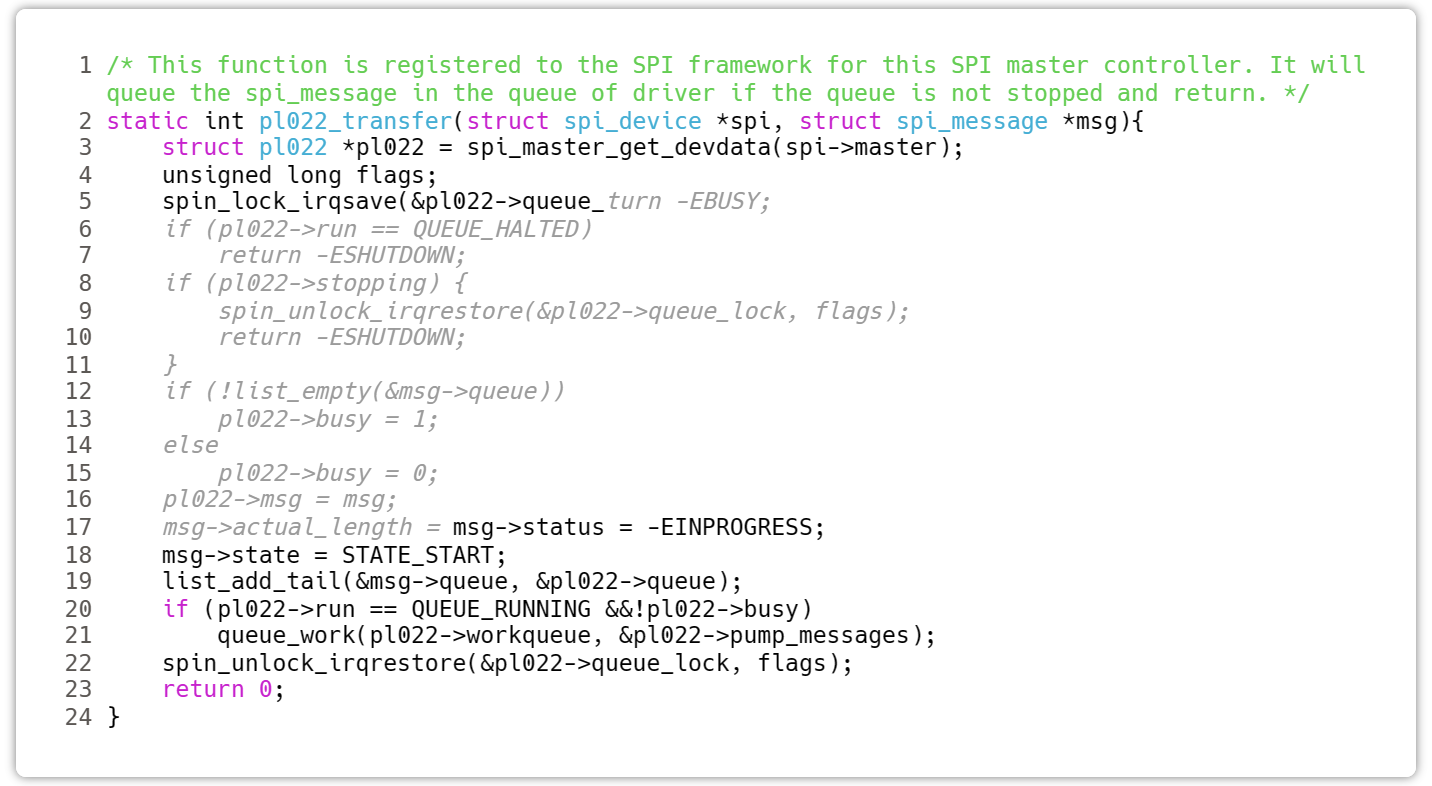
\includegraphics[width=0.9\textwidth]{obrazky/fim4.png}
    \caption{Model \MCfim{} má problém korektne naviazať na nasledujúci kód funkcie, ale je vidieť, že dobre zachytil kontext pred miestom vloženia nového kódu.}
    \label{code:MicroCoderFIM_1}
\end{figure}

Výsledky hodnotenia pass@k, uvedené v tabuľke~\ref{tab:humaneval-results} na dátovej sade HumanEval, poukazujú na to, že malý model po jeho ladení výrazne stratil schopnosť efektívne pracovať s jazykom Python. V porovnaní s pôvodným modelom \SC{} sú výsledky o~48\% nižšie. Ako ilustruje obrázok~\ref{fig:microcoderfim-python}, aj napriek poklesu výkonu model stále dokáže generovať korektný kód. Tento vývoj bol očakávaný vzhľadom na veľkosť modelu a je kľúčový pre posúdenie schopnosti modelu generalizovať na nové úlohy bez straty predtým nadobudnutých znalostí. Použil som $n=200$ výstupov na jeden príklad a parametre generovania sú $\text{temperature}=0,2$ a $\text{max\_new\_tokens}=128$. Pre inferenciu modelu som použil PSM formát techniky FIM. Ako prefix slúžilo zadanie z~dátovej sady. Sufix som nechal prázdny.

\begin{table}[!ht]
    \centering
    \begin{tabular}{r|c|c|c}
        \textbf{Model} & \textbf{pass@1} & \textbf{pass@10} & \textbf{pass@100} \\ \hline
        \MCfim{} & 7,83\,\% & 12,73\,\% & 19,07\,\% \\
    \end{tabular}
    \caption{Výsledky metrík pass@1, pass@10, pass@100 modelu \MCfim{} na dátovej sade HumanEval.}
    \label{tab:humaneval-results}
\end{table}

\begin{figure}[H]
    \centering
    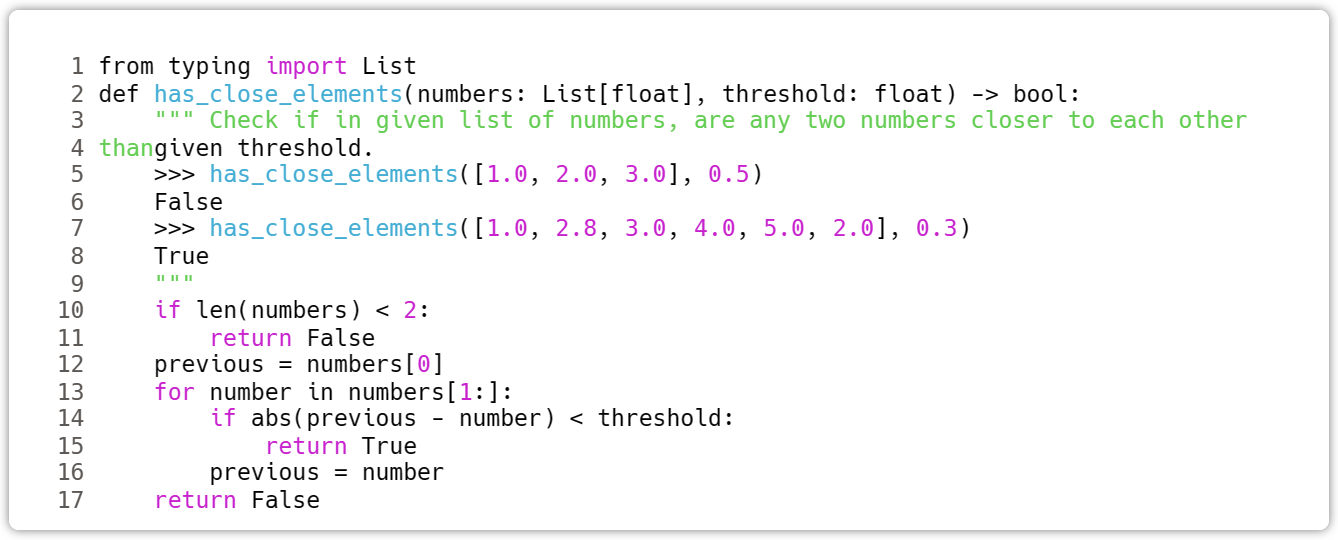
\includegraphics[width=0.9\textwidth]{obrazky/fim-python2.png}
    \caption{Výstup modelu \MCfim{} na zadanie z~dátovej sady HumanEval v~jazyku Python.}
    \label{fig:microcoderfim-python}
\end{figure}

\subsection{Rýchlosť inferencie}

Rýchlosť, akou model generuje kód, je dôležitým faktorom pri jeho použití v~reálnom prostredí. Preto som vyhodnotil rýchlosť inferencie modelov na testovacej sade. Každý model prešiel najprv fázou \uv{zohriatia} na jednom príklade a následne bol zmeraný čas generovania kódu 10-krát pre jednu vybranú vzorku. Výsledky sú zhrnuté v~tabuľke~\ref{tab:inference-speed}.

\begin{table}[!ht]
    \centering
    \small
    \begin{tabular}{c|c|c|c|c}
        \multirow{2}{*}{\textbf{Model}} & \textbf{Hĺbka} & \textbf{\O\,rýchlosť inferencie} & \textbf{\O\,čas inferencie } & \textbf{Max. nových} \\
        & [\textit{bit}] & [\textit{$token\cdot s^{-1}$}] & [\textit{s}] & \textbf{tokenov}\\
        \hline
        \multirow{3}{*}{\makecell{\textsc{CodeLlama-} \\ \textsc{Instruct 7B}}} & 16 & 2,18 & 92,3 & 512 \\
        & 8 & 10,98 & 38,30 & 512 \\
        & 4 & 32,61 & 12,10 & 512 \\
        \hline
        \MC{}& 4 & 32,82 & 10,99 & 512 \\
        \hline
        \makecell{\textsc{StarcoderBase}\\ \textsc{1B}}& 32 & 128 & $\pm 2,1$ & 256 \\
        \hline
        \MCfim{}& 32 & 128 & $\pm 2,1$ & 256 \\
    \end{tabular}
    \caption{Tabuľka rýchlosti inferencie modelov. Výsledky sú spriemerované hodnoty desiatich generácií výstupu pre jeden príklad. Porovnávané metriky sú priemerný čas inferencie a rýchlosť inferencie, ako počet tokenov vygenerovaný za jednotku času.}
    \label{tab:inference-speed}
\end{table}

Z~výsledkov je zrejmé, že kvanitizácia modelu zlepšila rýchlosť inferencie modelov. Nevýhodou je potenciálne zníženie kvality generovaného kódu. Rýchlosť inferencie modelu \MCfim{} je výrazne vyššia ako modelu \MC{}, čo je spôsobené menším počtom parametrov a rozdielnou implementáciou hláv pozornosti. Aj tieto výsledky ukazujú, že model \MCfim{} je vhodný pre použitie v~reálnom prostredí pri generovaní kódu a poskytovaní rýchlych nápovied programátorom. 

\chapter{Záver}\label{chap:conclusion}

V~tejto práci som sa venoval adaptácii predtrénovaných jazykových modelov na generovanie zdrojového kódu pre aplikácie vstavaných systémov. Práca sa sústredila na vytvorenie vhodnej dátovej sady zo zdrojových súborov v~jazykoch C a C++ a na následné ladenie modelov na novej dátovej sade s~cieľom optimalizovať ich výkonnosť.

V~úvodných kapitolách som predstavil základné princípy umelých neurónových sietí a architektúru transformer. Následne som sa venoval špecifikám použitia modelov hlbokého učenia v~oblasti NLP a generovania kódu. Zdôraznil som rozdiely medzi prirodzenými jazykmi a programovacími jazykmi, pričom som rozoberal ich syntaktické a sémantické osobitosti. Následne som sa zaoberal metodikou učenia veľkých jazykových modelov, metódami evaluácie ich generatívnych schopností a popísal som niekoľko existujúcich modelov.

V~implementačnej časti práce som popísal proces zberu dát a tvorbu novej dátovej sady. Vytvorená dátová sada obsahuje výber funkcií, z~rôznych projektov v~jazykoch C a C++, pre trénovanie jazykových modelov v~oblasti vstavaných systémov. Vykonal som analýzu vzoriek z~hľadiska ich veľkosti, štruktúry a navrhol spôsoby rozšírenia dátovej sady. Na vytvorenom korpuse dát som ladením vytvoril dva nové modely: \MC{} a \MCfim{}, určené na generovanie kódu špecificky pre oblasť vstavaných systémov. Popísal som proces ich trénovania, nastavené parametre a uhlíkovú stopu. Pri trénovaní modelu \MC{} som využil techniku kvantizácie váh a trénovania nízkorozmerných reprezentácií, za účelom optimalizácie výpočtových nárokov. Model \MCfim{} prešiel ladením všetkých váh modelu bez kvantizácie na upravenej dátovej sade technikou dopĺňania kódu v~kontexte.

Výsledky evaluácie modelov ukázali, že oba modely sú schopné generovať syntakticky správny a funkčne relevantný kód. Model \MCfim{} exceloval v~adaptácii na novú úlohu, čo dokázal výrazným zlepšením metrík po ladení. Tento model dokázal viac ako zdvojnásobiť efektívnosť pri generovaní kódu na dátovej sade po procese ladenia. Výsledky na metrike pass@k ukazujú, že \MCfim{} znížil schopnosť generovať kód v~jazyku Python a dosiahol skóre 7.83\,\% v metrike pass@1 na sade HumanEval. Vyhodnotil som tiež rýchlosť inferencie modelov, pričom \MCfim{} dosahuje násobne väčšiu rýchlosť generovania kódu vďaka implementácií MQA.

Na konci možno konštatovať, že ciele práce boli dosiahnuté. Zoznámil som sa s~využitím a adaptáciou jazykových modelov pre generovanie kódu, vytvoril som reprezentatívnu dátovú sadu komentovaných kódov a dva nové modely pre generovanie kódu. Budúce práce by mohli pokračovať v~rozširovaní dátového súboru použitím navrhovaných metód. Jednou z~možností je využitie smerníc MISRA-C na výber kvalitných trénovacích vzoriek.
%===============================================================================
% Pro kompilaci po částech (viz projekt.tex) nutno odkomentovat
%\end{document}